\documentclass[a4paper,12pt]{report}

% Pacotes (mantidos do template original do Insper, adequado para ABNT)
\usepackage[utf8]{inputenc}
\usepackage[T1]{fontenc}
\usepackage{graphicx}
\usepackage{amsmath}
\usepackage{amsfonts}
\usepackage{amssymb}
\usepackage{fancyhdr}
\usepackage{hyperref}
\usepackage{longtable}
\usepackage{tocbibind}
\usepackage{changepage}
\usepackage{geometry}
\usepackage{setspace}
\usepackage[portuguese]{babel}
\usepackage{caption}
\usepackage{ifthen}
\usepackage{times}
\usepackage[alf]{abntex2cite}
\usepackage[titles]{tocloft}
\usepackage{titlesec}
\usepackage{booktabs}
\usepackage[table]{xcolor}

% Cor usada para destacar a fonte de texto principal (nota de dívida
% isolada anual, confiável) em tabelas comparativas de fontes de texto.
\definecolor{fontechave}{RGB}{214,227,239}

% Cores usadas para destacar o modelo principal (M2) em tabelas de
% resultados por fonte de texto x grade M0-M3, e a interseção entre a
% coluna M2 e a linha da fonte principal (nota de dívida anual).
\definecolor{m2principal}{RGB}{253,236,209}
\definecolor{m2intersecao}{RGB}{233,231,224}

% Margens ABNT NBR 14724: superior 3cm, inferior 2cm, esquerda 3cm (encadernação), direita 2cm
\geometry{top=3cm, bottom=2cm, left=3cm, right=2cm}
\setlength{\parindent}{1.25cm}
\onehalfspacing

\renewenvironment{abstract}{
    \begin{center}
        \textbf{\abstractname}
    \end{center}
}{}

\titleformat{\chapter}[hang]
  {\normalfont\huge\bfseries}{\thechapter}{0.25em}{}

\addto\captionsportuguese{\renewcommand{\contentsname}{Sumário}}
\addto\captionsportuguese{\renewcommand{\bibname}{Referências}}

\title{Alterações textuais nas notas explicativas de dívida e a incorporação de informações pelo mercado brasileiro: evidências das notas de empréstimos, financiamentos e debêntures}
\author{Jonathan Mark Miranda Buscariolli Majoni}
\date{\the\year}
\newcommand{\advisor}{Ruy Monteiro Ribeiro}
% \newcommand{\coadvisor}{}

\begin{document}
\selectlanguage{portuguese}

\makeatletter

\begin{titlepage}
    \begin{minipage}[t]{0.35\textwidth}
        \raggedright
        
\includegraphics[width=0.7\textwidth]{Logo_Insper.png}
    \end{minipage}

    \vspace*{1.5cm}
    \centering
    {\large INSPER, INSTITUTO DE ENSINO E PESQUISA}\\[3cm]

    {\large \@author}\\[3cm]

    {\Large \textbf{\@title}}

    \vfill
    {\large São Paulo}\\
    {\large \the\year}
\end{titlepage}
\newpage

\begin{titlepage}
    \centering
    {\large \@author}\\[3cm]
    {\Large \textbf{\@title}}\\[3cm]

    \begin{adjustwidth}{7cm}{0cm}
        Dissertação apresentada ao Programa de Mestrado Profissional em Economia do Insper Instituto de Ensino e Pesquisa, como requisito parcial para obtenção do título de Mestre.

        \vspace*{0.5cm}
        Orientador(a): \advisor
        \ifcsname coadvisor\endcsname
            \\[0.25cm] Coorientador: \coadvisor
        \fi
    \end{adjustwidth}

    \vfill
    {\large São Paulo}\\
    {\large \the\year}
\end{titlepage}
\newpage

% Na versão final: Ficha catalográfica (biblioteca) e Folha de aprovação (pós-defesa) entram aqui.
% Não incluídas nesta versão por dependerem de processos institucionais externos.

\thispagestyle{empty}
\newpage

\renewcommand{\abstractname}{Resumo}
\begin{abstract}
    Utilizando um painel de 185 empresas não financeiras que integram ou já integraram o índice IBX da B3 entre 2010 e 2025, mostramos que a mudança textual ano a ano na nota explicativa de empréstimos, financiamentos e debêntures está associada ao retorno anormal futuro das ações, mesmo após controlar pelas mudanças nos fundamentos econômico-financeiros da empresa. O efeito é estatisticamente significativo em toda a grade de controles testada ($\beta=0{,}156$; $p=0{,}017$ na especificação principal) e é corroborado por dois métodos de identificação independentes: um teste de portfólio calendário (alfa de $-11{,}4\%$ ao ano; $p=0{,}0011$) e uma especificação alternativa de efeitos, selecionada por teste de Hausman ($p=0{,}043$ a $0{,}080$). É a única, entre quatro fontes de texto testadas como checagem de especificidade e generalização, a mostrar esse padrão -- consistente com a teoria de atenção limitada, já que a nota de dívida é a mais técnica e menos discricionária das quatro. A mudança textual é medida por TF-IDF e similaridade de cosseno entre o texto da nota de um exercício e a do exercício anterior, seguindo a abordagem de \citeonline{cohen2020} e \citeonline{brown2011}; o retorno anormal é medido como o resíduo fora da amostra de um modelo de quatro fatores (mercado, tamanho, valor e momento) estimado por empresa, acumulado numa janela de doze meses e ajustado por winsorização, com controles organizados em uma grade pré-especificada de blocos cumulativos (fundamentos de nível, mudanças contemporâneas nesses fundamentos, e determinantes de risco e retorno esperado), estimada em painel com efeitos fixos de empresa e ano e erros-padrão agrupados por empresa.
\end{abstract}

\vspace{0.5cm}
\noindent
\textbf{Palavras-chave:} notas explicativas; análise textual; TF-IDF; retorno anormal; BHAR; modelo de quatro fatores; dados em painel; disclosure; consenso de estimativas.
\thispagestyle{empty}
\newpage

\renewcommand{\abstractname}{Abstract}
\selectlanguage{english}
\begin{abstract}
    Using a panel of 185 non-financial companies that are or have been constituents of B3's IBX index between 2010 and 2025, we show that year-over-year textual change in the explanatory note on loans, financing, and debentures is associated with firms' future abnormal stock returns, even after controlling for changes in the firm's economic and financial fundamentals. The effect is statistically significant across the whole control grid tested ($\beta=0.156$; $p=0.017$ in the principal specification) and is corroborated by two independent identification methods: a calendar-time portfolio test (annualized alpha of $-11.4\%$; $p=0.0011$) and an alternative, Hausman-selected effects specification ($p=0.043$ to $0.080$). It is the only one of four text sources tested as a specificity and generalization check to show this pattern -- consistent with limited-attention theory, since the debt note is the most technical and least discretionary of the four. Textual change is measured via TF-IDF and cosine similarity between the note's text in a given fiscal year and the previous year, following the approach of Cohen, Malloy and Nguyen (2020) and Brown and Tucker (2011); abnormal returns are measured as the out-of-sample residual from a firm-level four-factor model (market, size, value, and momentum), accumulated over a twelve-month window and adjusted via winsorization, with controls organized into a pre-specified grid of cumulative blocks (level fundamentals, contemporaneous changes in those fundamentals, and risk/expected-return determinants), estimated in a panel with company and year fixed effects and firm-clustered standard errors.
\end{abstract}

\vspace{0.5cm}
\noindent
\textbf{Keywords:} explanatory notes; textual analysis; TF-IDF; abnormal returns; BHAR; four-factor model; panel data; disclosure; analyst consensus estimates.
\selectlanguage{portuguese}
\thispagestyle{empty}
\newpage

\tableofcontents
\thispagestyle{empty}
\newpage

\chapter{Introdução}

Nem toda informação relevante é lida com a mesma atenção. A teoria de atenção limitada mostra que o investidor reage rápido a informação saliente -- o lucro do trimestre, o release, a teleconferência -- mas reage devagar, ou não reage, a informação tecnicamente densa e pouco divulgada, mesmo quando essa informação é, ela mesma, relevante para o risco da empresa \cite{hirshleifer2011}. Esta dissertação testa essa ideia num lugar específico e pouco explorado: a nota explicativa de empréstimos, financiamentos e debêntures. É ali que vencimento, taxa, garantia, covenant e renegociação -- os termos que determinam se uma empresa consegue honrar ou rolar sua dívida -- estão descritos; o saldo agregado da dívida, sozinho, não carrega essa informação. Mas é também um dos pedaços mais técnicos e menos lidos de um pacote de divulgação de 30 a 150 páginas, disputando atenção do investidor com o lucro, o EBITDA, o release e a teleconferência do mesmo trimestre. Informação real e atenção mínima: essa combinação é exatamente onde a teoria prevê que o mercado demore mais para incorporar preço -- e é essa previsão específica, não apenas ``o texto muda de um ano para o outro'', que esta dissertação testa.

A pergunta, formalmente: empresas cuja nota de empréstimos, financiamentos e debêntures muda mais, de um exercício para o outro, têm retorno anormal diferente nos doze meses seguintes à divulgação, mesmo depois de controlar pelas mudanças observáveis nos fundamentos da empresa? A mudança textual é medida por TF-IDF e similaridade de cosseno entre o texto da nota em dois exercícios consecutivos -- a mesma lógica de \citeonline{brown2011} e de \citeonline{cohen2020} (``Lazy Prices''), que encontram, para o mercado americano, que empresas cujos documentos regulatórios mudam mais no texto têm desempenho futuro pior, sem reação imediata de preço na data de divulgação. O recorte para a nota de dívida especificamente, e não o documento inteiro, é a escolha estrutural desta dissertação, e vem de uma evidência direta do próprio mecanismo de atenção limitada: \citeonline{amelzadeh2016} comparam o texto do relatório da administração (MD\&A) com o das notas explicativas de um 10-K americano e encontram que o mercado reage rápido e forte ao MD\&A -- mas que mudanças no texto das notas, o pedaço mais técnico do pacote, preveem retorno futuro e desempenho operacional, sinal de que a informação ali demora mais para ser precificada. Se esse mecanismo existe, a nota de dívida -- e não o relatório da administração, mais lido e mais discutido -- é o lugar certo para testá-lo. É também uma pergunta ainda não respondida no Brasil: a literatura nacional sobre notas explicativas cobre legibilidade \cite{borges,silva2019}, tom \cite{muniz2025}, covenants \cite{schiozer2021} e, mais recentemente, um índice de informatividade construído com modelo de linguagem \cite{costaneto2025}, mas nenhum desses trabalhos testa se a mudança textual ano a ano, medida de forma simples e replicável, prevê retorno futuro.

O resultado principal, em uma frase: sim, e exatamente onde a teoria previa. Sobre uma amostra de 185 empresas não financeiras listadas na B3 e 1.134 pares empresa-ano (2010--2025), a mudança textual da nota de dívida anual está associada ao retorno anormal futuro de forma estatisticamente significativa a 5\% em toda a grade de controles testada, do diagnóstico simples ($p=0{,}010$) até a especificação com controles completos ($p=0{,}011$), passando pela especificação principal pré-especificada ($\beta=0{,}156$, $p=0{,}017$). O coeficiente sobrevive a exclusão de escores de similaridade degenerados, ao BHAR sem winsorização e à exclusão de cada empresa individualmente (Seção~\ref{sec:robustez}) -- não é um artefato de uma especificação isolada ou de uma empresa influente. Dois métodos de identificação inteiramente diferentes da regressão em painel corroboram a mesma direção: um teste de portfólio calendário longo-curto encontra um alfa de quatro fatores de $-11{,}4\%$ ao ano ($p=0{,}0011$), e reestimar o modelo sob o desenho de \citeonline{santoscoelho2018} (efeito único de empresa, escolhido por teste de Hausman) também rejeita a hipótese nula ($p=0{,}043$ a $0{,}080$, dependendo da janela). Mas o resultado vem com uma qualificação que esta dissertação não suaviza: entre quatro fontes de texto testadas (o conjunto completo de notas explicativas, o Relatório da Administração, os Fatores de Risco do Formulário de Referência), usadas como checagens de especificidade e generalização, e não como testes confirmatórios independentes da mesma hipótese, é a única a atingir significância a 5\% em toda a grade M0-M3.

E a especificidade do resultado é, ela mesma, parte do achado. Entre as quatro fontes de texto testadas, a nota de dívida é a mais técnica e a mais auditada -- a menos discricionária, a mais parecida com boilerplate contábil de um ano para o outro. É justamente nela, e somente nela, que o efeito aparece: nem no Relatório da Administração (o texto mais lido e mais discursivo do pacote), nem nos Fatores de Risco do Formulário de Referência. Esse padrão é exatamente o que a teoria de atenção limitada prevê e é a confirmação mais direta do mecanismo que motiva esta dissertação -- o mesmo padrão que \citeonline{amelzadeh2016} documentam para o mercado americano (notas preveem retorno futuro, MD\&A não). Ele diverge, por outro lado, da heterogeneidade interna reportada por \citeonline{cohen2020}, que encontram o efeito concentrado em texto de maior discricionariedade gerencial (Risk Factors, MD\&A) dentro da própria amostra americana. Essa divergência entre dois estudos que motivam esta dissertação -- não a significância em si -- é o que há de mais informativo aqui sobre onde e como a atenção limitada opera no mercado brasileiro, e é retomada com mais profundidade no Capítulo~\ref{ch:conclusao}.

A contribuição desta dissertação, portanto, tem três partes. Primeiro, e mais diretamente ligada ao resultado acima: ela testa, com desenho pré-especificado antes de qualquer resultado, se a atenção limitada se manifesta especificamente na seção mais técnica e menos lida de um pacote de divulgação financeira -- não apenas ``o texto muda'', mas muda exatamente onde a teoria diz que o mercado deveria demorar mais para perceber. Segundo, ela testa essa pergunta pela primeira vez no Brasil com o recorte específico de notas de dívida: a literatura brasileira sobre notas explicativas, revisada no Capítulo~\ref{ch:referencial}, chega perto (legibilidade, tom, covenants) sem fazer esse teste, e a pergunta já respondida para o mercado americano por \citeonline{cohen2020} e \citeonline{brown2011} nunca havia sido replicada aqui com esse recorte. Terceiro, ela usa como variável dependente um modelo de quatro fatores com alfa próprio por empresa (Seção~\ref{sec:var_dependente}), mais alinhado à tradição de \citeonline{barberlyon1997} para retorno anormal de longo prazo do que o retorno simplesmente ajustado ao índice usado em versões exploratórias anteriores deste projeto, testado sob uma grade de controles pré-especificada (M0-M3, Seção~\ref{sec:controles}) e corroborado por dois métodos de identificação independentes -- um padrão de evidência mais completo do que uma única regressão significativa.

\section{Hipóteses}
\label{sec:hipoteses}

\textbf{H1}: as alterações textuais entre exercícios nas notas de empréstimos, financiamentos e debêntures estão associadas ao retorno anormal futuro das ações, mesmo depois de controlar pelas mudanças observáveis nos fundamentos da empresa. A hipótese é mantida sem direção definida de propósito: uma mudança grande no texto pode originar de uma notícia ruim (quebra de covenant, dificuldade de refinanciamento) ou de uma notícia boa (alongamento de prazo, redução de taxa, quitação de dívida), e não se pode assumir de antemão qual predomina. Essa leitura segue \citeonline{brown2011}: o teste central usa a \emph{magnitude} da reação de preço ao texto modificado, não sua direção.

\textbf{H1a} (exploratória): empresas com maior mudança textual nas notas de dívida apresentam retorno anormal futuro \emph{menor}, na linha do que \citeonline{cohen2020} encontram para o mercado americano. Só se sustenta se a mudança estiver concentrada em notícia desfavorável; tratada como teste adicional, não como hipótese central.

\textbf{H2} (complementar): as alterações textuais nas notas de dívida também se associam à revisão do consenso de EPS dos analistas depois da divulgação.

\section{Estrutura da dissertação}

O Capítulo~\ref{ch:referencial} monta o argumento teórico por trás do desenho: por que atenção limitada prevê sub-reação especificamente em texto técnico, por que mudança (e não nível) é a forma certa de medir informação nova, e por que a nota de dívida é onde essa mudança deveria importar mais. O Capítulo~\ref{ch:metodologia} descreve a coleta e extração das notas, a medida de mudança textual, a variável dependente (BHAR ajustado sobre um modelo de quatro fatores), a grade de controles M0-M3 e a estratégia de identificação, incluindo as três ameaças à inferência endereçadas (observações repetidas, variável omitida no nível da empresa, causalidade reversa) e como cada uma é tratada. O Capítulo~\ref{ch:dados} descreve a amostra final, as quatro fontes de texto e três fontes de dados estruturados combinadas, e a confiabilidade da extração. O Capítulo~\ref{ch:resultados} reporta os resultados de H1 e H2 para cada fonte de texto e a bateria de robustez do resultado principal. O Capítulo~\ref{ch:conclusao} discute as leituras alternativas para o padrão de resultados encontrado, suas limitações, e os próximos passos identificados ao longo do trabalho.

\chapter{Referencial Teórico}
\label{ch:referencial}

Este capítulo monta, em três passos, o argumento por trás do desenho da Introdução: por que atenção limitada prevê um efeito especificamente em texto técnico e pouco lido (Seção~\ref{sec:atencao}); por que medir \emph{mudança}, e não o nível de um documento, é a forma certa de isolar informação nova em texto cheio de boilerplate (Seção~\ref{sec:mudanca_sinal}); e por que a nota de dívida, especificamente, é onde a literatura sobre divulgação e mercado de crédito diz que essa mudança deveria importar mais (Seção~\ref{sec:divida_credito}). A Seção~\ref{sec:lacuna} fecha o capítulo situando essa dissertação contra o que já existe no Brasil.

\section{Atenção limitada: por que texto técnico é onde a teoria prevê sub-reação}
\label{sec:atencao}

A base teórica mais geral é a assimetria de informação entre os administradores, que acompanham de perto a operação da empresa, e os investidores de fora, que dependem do que é publicado -- divulgação pública reduz essa assimetria e pode aumentar liquidez e reduzir custo de capital \cite{diamond1991}, e demonstrações financeiras, auditoria, intermediários de informação e divulgação voluntária são os mecanismos pelos quais o mercado tenta resolvê-la \cite{healy2001}. Mas assimetria de informação, por si só, não explica \emph{quando} o mercado processa uma informação já publicada -- só explica por que ela precisa ser publicada. A peça que falta é atenção: \citeonline{hirshleifer2011} desenvolvem um modelo em que a atenção limitada dos investidores explica tanto sub-reação quanto sobre-reação a diferentes componentes da informação contábil, dependendo de quão saliente cada componente é. Informação saliente (o lucro do trimestre, o release, a teleconferência) é processada rápido; informação tecnicamente densa e pouco divulgada -- mesmo quando relevante para o risco da empresa -- pode demorar mais para ser incorporada ao preço, simplesmente porque poucos investidores a leem com cuidado no momento da divulgação.

É esse mecanismo, não a assimetria de informação isoladamente, que torna a nota de dívida um objeto de estudo interessante. Ela não é apenas mais uma fonte de informação relevante -- vencimento, taxa, garantia, covenant e renegociação, os termos que determinam se a empresa consegue honrar ou rolar sua dívida, não aparecem no saldo agregado do balanço, só no texto da nota --; ela é, especificamente, um candidato a informação relevante processada com atraso, por estar entre os pedaços mais técnicos e menos lidos de um pacote de divulgação de 30 a 150 páginas, competindo por atenção com o lucro líquido, o EBITDA, o release e a teleconferência do mesmo trimestre. A evidência mais direta de que esse mecanismo realmente separa seções de um mesmo documento vem de \citeonline{amelzadeh2016}: comparando o texto do relatório da administração (MD\&A) com o das notas explicativas em formulários 10-K americanos, os autores encontram que a reação dos investidores é mais rápida e mais forte para o MD\&A do que para as notas, e que mudanças no texto das notas -- não no MD\&A -- predizem retorno futuro e desempenho operacional. Ou seja: dentro do mesmo arquivamento, a seção mais lida é precificada rápido, e a seção mais técnica carrega previsibilidade que sobra para depois. É esse resultado, especificamente, que justifica escolher a nota de dívida -- e não o relatório da administração, mais lido e mais discutido -- como objeto central desta dissertação (Seção~\ref{sec:medida}).

\section{Mudança textual como sinal de informação nova}
\label{sec:mudanca_sinal}

Documento financeiro tem muito texto repetido. Política contábil, descrição de contrato e trecho normativo podem ficar praticamente iguais por vários anos seguidos, o que significa que o \emph{nível} de uma medida textual (por exemplo, quantas palavras negativas a nota tem) não separa bem texto estrutural repetitivo de informação nova do exercício -- uma nota antiga e uma nova podem ter o mesmo nível de "negatividade" sem que nada tenha mudado de fato. \citeonline{brown2011} resolvem esse problema comparando a seção MD\&A de cada empresa com a do ano anterior, e mostram que a \emph{mudança} de um ano para o outro está associada a mudanças econômicas reais e à reação dos preços -- não o nível do texto em si. \citeonline{cohen2020}, no estudo conhecido como Lazy Prices, ampliam essa lógica para o histórico completo de documentos regulatórios (10-K e 10-Q) de empresas americanas: empresas cujos documentos mudam mais no texto têm desempenho futuro pior do que empresas cujos documentos ficam parecidos ano após ano, sem reação de mercado imediata na data da divulgação -- consistente com desatenção dos investidores à mudança textual em si, o mesmo mecanismo de atenção limitada da Seção~\ref{sec:atencao}, agora medido pela comparação ano a ano em vez de pela comparação entre seções de um mesmo documento.

É essa literatura que sustenta a medida usada nesta dissertação:
\begin{align}
    \text{Similaridade}(i,t) &= \cos\left(\mathit{TFIDF}(i,t), \mathit{TFIDF}(i,t-1)\right) \\
    \text{Mudança textual}(i,t) &= 1 - \text{Similaridade}(i,t)
\end{align}
A medida capta mudança lexical, isto é, alterações nas palavras e expressões utilizadas, não necessariamente mudança de significado: duas frases semanticamente equivalentes, mas redigidas com vocabulário distinto, produziriam baixa similaridade de cosseno mesmo na ausência de mudança econômica real. Por isso, a variável é denominada mudança textual ou lexical ao longo desta dissertação, evitando termos como ``novidade semântica'', que sugeririam uma precisão que o método não possui.

\section{Divulgação de dívida e resultados de mercado}
\label{sec:divida_credito}

Se atenção limitada explica \emph{quando} o mercado processa informação técnica, falta ainda mostrar que a nota de dívida especificamente -- e não qualquer seção técnica qualquer -- carrega informação com peso real sobre risco e retorno. Dois estudos internacionais ligam diretamente a qualidade textual da divulgação a resultados no mercado de dívida: \citeonline{ertugrul2017} mostram que relatórios anuais menos legíveis e com tom mais ambíguo se associam a cláusulas de empréstimo mais restritivas e a maior risco futuro de queda abrupta no preço da ação; \citeonline{bonsall2017} mostram que menor legibilidade das divulgações narrativas se associa a ratings de crédito menos favoráveis e a mais divergência entre agências de rating. Os dois reforçam que o pedaço da divulgação relacionado à dívida é especialmente sensível à qualidade da comunicação textual -- não um recorte arbitrário entre vários possíveis.

No Brasil, essa relevância já foi confirmada diretamente no nível do conteúdo, não apenas por inferência da literatura internacional: \citeonline{schiozer2021} mostram, com coleta manual em milhares de notas de empréstimos e financiamentos de empresas da B3, que essas notas carregam informação contratual concreta sobre covenants. Entre a evidência internacional de que texto de dívida move mercado de crédito e a confirmação brasileira de que a nota especificamente carrega conteúdo contratual real, o recorte desta dissertação -- a nota, e não o documento inteiro, como unidade de análise -- fica duplamente justificado.

\section{Panorama brasileiro e a lacuna que a pesquisa ocupa}
\label{sec:lacuna}

A literatura nacional sobre notas explicativas cobre bem legibilidade \cite{borges,silva2019}, tom e crise \cite{muniz2025}, mineração de texto em notas de risco de instituições financeiras \cite{marcolin}, previsão de variação de indicador contábil a partir de texto de notas \cite{maeda2017}, conformidade com IFRS e erro de previsão de analista \cite{santos2018}, covenants em notas de dívida \cite{schiozer2021}, e, mais recentemente, um índice sofisticado de informatividade construído com modelo de linguagem em português \cite{costaneto2025}, ainda sem validação contra variável de mercado. Nenhum desses trabalhos, porém, testa se a mudança textual ano a ano, medida de forma simples e replicável nas notas de dívida, carrega informação a mais sobre o retorno futuro das ações ou sobre a revisão das previsões dos analistas -- é essa a lacuna específica que esta dissertação ocupa, apoiada em literatura internacional já consolidada sobre atenção limitada e mudança textual \cite{cohen2020,amelzadeh2016,brown2011}.

\chapter{Metodologia}
\label{ch:metodologia}

\section{Coleta e extração das notas explicativas}
\label{sec:coleta}

As notas explicativas foram coletadas diretamente do portal de dados abertos da CVM (DFP, Demonstrações Financeiras Padronizadas anuais), a partir dos pacotes de arquivamento (\textit{filing packages}) de cada empresa-exercício. A nota específica de empréstimos, financiamentos e debêntures é isolada dentro do documento completo de notas explicativas (tipicamente 30--150 páginas) por meio de uma heurística baseada em metadados de layout do PDF (tamanho de fonte, negrito, posição), não apenas por expressão regular sobre o texto, o que é necessário porque as mesmas palavras-chave aparecem em sumários, referências cruzadas e menções incidentais no corpo do texto, não apenas no título real da seção. A confiabilidade dessa extração e a cobertura obtida para cada fonte de texto são detalhadas no Capítulo~\ref{ch:dados}.

\section{Medida de mudança textual (TF-IDF e similaridade de cosseno)}
\label{sec:medida}

A mudança textual é medida por 1 menos a similaridade de cosseno entre os vetores TF-IDF do texto da nota em dois exercícios consecutivos da mesma empresa. Como essa medida é a base empírica de toda a dissertação, vale detalhar sua mecânica antes de descrever como ela é aplicada aqui.

\textbf{TF-IDF.} A sigla vem do inglês \textit{Term Frequency-Inverse Document Frequency}, e resume duas informações sobre cada palavra de um documento. A primeira, TF (frequência do termo), é simplesmente quantas vezes uma palavra aparece no texto, normalizada pelo tamanho do documento para não favorecer notas apenas por serem mais longas. A segunda, IDF (frequência inversa nos documentos), penaliza palavras comuns e valoriza palavras raras, de acordo com a fórmula
\begin{equation}
    \mathit{IDF}(palavra) = \log\left(\frac{N}{\text{número de documentos que contêm a palavra}}\right),
    \label{eq:idf}
\end{equation}
em que $N$ é o número total de documentos do corpus. Se uma palavra aparece em praticamente toda nota de dívida do setor (``empréstimo'', ``taxa'', ``vencimento'', ``garantia''), o denominador se aproxima de $N$, a razão se aproxima de 1 e o logaritmo se aproxima de zero: o IDF é baixo, e a palavra quase não pesa no resultado final, por mais vezes que se repita. Se a palavra aparece em pouquíssimos documentos (o nome de um banco credor específico, uma cláusula de covenant incomum), o IDF é alto, e ela passa a pesar bem mais. O peso final de cada palavra em cada documento é o produto das duas partes, $\mathit{TF\text{-}IDF} = \mathit{TF} \times \mathit{IDF}$: alto quando a palavra é frequente naquele texto específico \emph{e} rara no corpus como um todo, baixo quando qualquer uma das duas condições falha. Cada nota, assim, deixa de ser um bloco de texto e passa a ser um vetor numérico, com uma posição para cada palavra do vocabulário do corpus (tipicamente milhares de posições, a maioria delas zero).

\textbf{Similaridade de cosseno.} Com cada nota já representada como um vetor, a pergunta seguinte é o quão parecidos são o vetor do exercício $t$ e o vetor do exercício $t-1$ da mesma empresa. A similaridade de cosseno mede o ângulo entre os dois vetores, não a distância bruta entre eles:
\begin{equation}
    \cos(A,B) = \frac{A \cdot B}{\lVert A \rVert \, \lVert B \rVert},
    \label{eq:cosseno}
\end{equation}
em que $A \cdot B$ é o produto escalar dos dois vetores e $\lVert A \rVert$, $\lVert B \rVert$ são suas normas. Como os pesos TF-IDF nunca são negativos, o resultado varia de 0 a 1 neste contexto: 1 significa que os dois vetores apontam exatamente na mesma direção, ou seja, a mesma proporção relativa de palavras-chave nos dois exercícios (nota praticamente reciclada de um ano para o outro); 0 significa nenhuma sobreposição relevante de vocabulário entre os dois anos. A vantagem de usar cosseno em vez de, por exemplo, distância euclidiana, é que ele ignora o tamanho do documento e depende só da direção do vetor: uma nota pode crescer ou encolher de um ano para o outro sem necessariamente mudar de conteúdo (mais tabelas de detalhamento sobre o mesmo assunto, por exemplo), e o cosseno não confunde ``documento maior'' com ``documento diferente''.

Com a nota já representada dessa forma nos dois exercícios, a mudança textual usada nesta dissertação é definida como o complemento da similaridade, $1 - \cos(A,B)$: quanto mais próxima de 1 a similaridade, menor a mudança; quanto mais próxima de 0, maior. O vocabulário e os pesos IDF são ajustados uma única vez sobre todo o corpus da amostra, não empresa a empresa, para que a ponderação reflita o que é de fato boilerplate genérico do setor e do mercado como um todo, e não apenas o que se repete para uma única empresa ao longo do tempo. A ponderação TF-IDF especificamente segue \citeonline{brown2011}, que a adotam sobre o modelo de espaço vetorial clássico da literatura de recuperação de informação por sua simplicidade e popularidade. \citeonline{cohen2020} usam uma medida de cosseno análoga, mas sobre vetores de frequência bruta de termos, sem a ponderação por raridade que caracteriza o TF-IDF; a escolha desta dissertação segue a variante de \citeonline{brown2011}, por permitir separar melhor o boilerplate setorial da mudança de fato específica de cada empresa.

Ajustar o IDF sobre o corpus inteiro, incluindo exercícios futuros em relação a cada par ano a ano, levanta uma preocupação legítima de \textit{look-ahead}: a representação de uma nota de 2016, por exemplo, é influenciada pela frequência de palavras observada em notas de 2024, informação que não existia no momento da divulgação de 2016. A Seção~\ref{sec:robustez} testa diretamente essa preocupação, recalculando o IDF em janela expansiva (usando, para cada par, apenas documentos disponíveis até o exercício corrente) e reestimando H1 sobre a similaridade resultante.

\section{Variável dependente: retorno anormal futuro}
\label{sec:var_dependente}

O retorno anormal é medido como o resíduo, fora da amostra, de um modelo de fatores estimado por empresa, na tradição metodológica descrita por \citeonline{barberlyon1997} para estudos de retorno anormal de longo prazo.

\textbf{Modelo de quatro fatores.} Para cada evento (par empresa-exercício com mudança textual computável), estima-se um modelo de fatores ao estilo \citeonline{carhart1997} -- o modelo de três fatores de \citeonline{famafrench1992} acrescido de um quarto fator de momento, na tradição documentada por \citeonline{jegadeeshtitman1993} --, numa janela de estimação de 252 pregões (aproximadamente 12 meses) que termina estritamente antes do início da janela de evento, sem sobreposição:
\begin{equation}
    R_{i,d} - R_{f,d} = \alpha_i + \beta_M \mathit{MKT}_d + \beta_S \mathit{SMB}_d + \beta_H \mathit{HML}_d + \beta_{Mom} \mathit{MOM}_d + \varepsilon_{i,d},
    \label{eq:fatores}
\end{equation}
em que $R_{i,d}$ é o retorno diário da ação $i$, $R_{f,d}$ a taxa livre de risco, e $\mathit{MKT}$, $\mathit{SMB}$, $\mathit{HML}$ e $\mathit{MOM}$ os fatores de mercado, tamanho, valor e momento para o mercado brasileiro, publicados pelo NEFIN/USP \cite{nefin2026}. Diferentemente do CAPM (que usa apenas $\mathit{MKT}$), o modelo de quatro fatores permite que o retorno esperado da ação reflita também sua exposição a tamanho, valor e momento, dimensões que a literatura de \textit{asset pricing} associa a variação relevante no retorno médio das ações \cite{famafrench1992}.

\textbf{Retorno anormal como resíduo fora da amostra.} O alfa $\alpha_i$ e os betas estimados na equação~\ref{eq:fatores} definem o desempenho ``normal'' de cada empresa: seu retorno médio esperado, dado o que aconteceu com os quatro fatores em cada dia. O retorno anormal na janela de evento (os 12 meses seguintes à divulgação) é o desvio, dia a dia, entre o retorno realmente observado e esse desempenho esperado, calculado com os parâmetros já fixados na janela de estimação anterior -- ou seja, fora da amostra usada para estimá-los:
\begin{equation}
    \varepsilon_{i,d}^{evento} = \left(R_{i,d} - R_{f,d}\right) - \left(\hat\alpha_i + \hat\beta_M \mathit{MKT}_d + \hat\beta_S \mathit{SMB}_d + \hat\beta_H \mathit{HML}_d + \hat\beta_{Mom} \mathit{MOM}_d\right).
    \label{eq:residuo_evento}
\end{equation}
Note que $\hat\alpha_i$ permanece na conta: o desempenho idiossincrático médio da própria empresa durante a janela de estimação é tratado como parte do ``normal'' dessa empresa, e só o desvio em relação a esse próprio referencial conta como retorno anormal -- uma diferença deliberada em relação a um modelo de fatores sem alfa, que trataria qualquer desempenho idiossincrático médio da empresa como já ``anormal'' por definição.

\textbf{BHAR.} Os resíduos diários da janela de evento são agregados numa única medida por evento compondo-os multiplicativamente, não somando-os: o BHAR (\textit{Buy-and-Hold Abnormal Return}), que replica o que um investidor realmente experimentaria comprando e mantendo a posição pelos 12 meses da janela:
\begin{equation}
    \mathit{BHAR}_i = \prod_{d=1}^{D}\left(1 + \varepsilon_{i,d}^{evento}\right) - 1.
    \label{eq:bhar}
\end{equation}
\citeonline{barberlyon1997} defendem essa composição multiplicativa como mais fiel ao ganho econômico real de uma estratégia de longo prazo do que uma soma aritmética dos resíduos diários, e é essa fidelidade ao que o investidor de fato experimenta que justifica adotar o BHAR aqui. Mas tanto eles quanto \citeonline{fama1998} documentam um problema estatístico associado à composição multiplicativa: como o retorno de uma ação é limitado em $-100\%$ mas ilimitado para cima, compor retornos diários ao longo de uma janela de 12 meses produz uma distribuição fortemente assimétrica à direita, mesmo na ausência de qualquer sinal real -- um problema que se agrava em amostras pequenas e que \citeonline{lyonbarbertsai1999} tratam formalmente, propondo testes ajustados por assimetria e métodos de \textit{bootstrap} como correção. Nesta amostra (nota de dívida anual, $n=1.134$), a assimetria do BHAR bruto é de $9{,}33$ -- muito acima do que testes paramétricos usuais (como a regressão por MQO agrupada por empresa usada em toda a dissertação, Seção~\ref{sec:identificacao}) pressupõem sem ajuste.

\textbf{BHAR ajustado.} Em vez de um teste ajustado por assimetria (desenhado originalmente para comparação de médias entre dois grupos, não para regressão multivariada), adotou-se a correção mais direta: a winsorização do BHAR nos percentis 1 e 99, que reduz a assimetria da amostra de $9{,}33$ para $1{,}88$ sem descartar nenhuma observação. Essa medida -- BHAR ajustado -- é a variável dependente usada em toda regressão reportada a partir daqui.

Os betas estimados na equação~\ref{eq:fatores} são plausíveis, com beta de mercado tipicamente próximo de 1 na amostra completa de eventos, consistente com uma carteira de ações do próprio índice de referência. Um mínimo de 100 observações diárias válidas é exigido na janela de estimação; eventos que não atingem esse mínimo são descartados.

\section{Variáveis de controle: grade M0-M3}
\label{sec:controles}

As variáveis de controle foram organizadas ex ante em blocos cumulativos (M0 a M3), definidos e documentados antes da rodada de estimações que gerou os resultados do Capítulo~\ref{ch:resultados}.

\textbf{M0 -- diagnóstico.} Apenas TextChange, com efeitos fixos de empresa e ano (Seção~\ref{sec:modelo}). Não é interpretado como o teste de conteúdo informacional incremental; estabelece o comportamento do coeficiente antes da entrada dos blocos de fundamentos, para que a comparação com M1-M3 seja informativa.

\textbf{M1 -- fundamentos clássicos (\textit{baseline}).} Acrescenta tamanho (logaritmo do ativo total), rentabilidade (ROA, lucro líquido sobre ativo total), alavancagem (passivo total sobre ativo total) e momento (retorno acumulado dos 12 meses anteriores à divulgação). Tamanho e \textit{momentum} têm respaldo direto em \citeonline{famafrench1992}, que mostram que tamanho captura variação relevante na seção transversal de retornos médios, e em \citeonline{jegadeeshtitman1993}, que documentam persistência de desempenho em estratégias formadas por retorno passado em horizontes de 3 a 12 meses -- horizonte compatível com a janela usada aqui. ROA e alavancagem seguem \citeonline{santos2018}, que os utilizam como controle em modelo de erro de previsão de analistas no contexto brasileiro; alavancagem é um controle particularmente relevante por aproximar diretamente risco financeiro e estrutura de capital.

\textbf{M2 -- mudança nos fundamentos (\textbf{modelo principal}).} Acrescenta a variação, entre o exercício $t-1$ e o exercício $t$, de ROA ($\Delta\mathit{ROA}$), de alavancagem ($\Delta\mathit{Alavancagem}$) e de dívida ($\Delta\mathit{Dívida}$, mudança na conta específica de empréstimos, financiamentos e debêntures, normalizada pelo ativo total do exercício anterior). A variável de interesse, TextChange, é por construção uma mudança entre $t-1$ e $t$; controlar apenas o \emph{nível} dos fundamentos em M1 deixa aberta a possibilidade de TextChange estar funcionando como um proxy para mudanças econômicas contemporâneas, não para conteúdo textual incremental. \citeonline{brown2011} tornam essa preocupação concreta ao mostrar que firmas com maiores mudanças econômicas modificam mais sua narrativa: se a nota mudou simplesmente porque a empresa tomou, amortizou ou refinanciou dívida, TextChange pode estar capturando essa alteração já observável em $\Delta\mathit{Dívida}$, não informação adicional. M2 é, portanto, o modelo que mais fielmente traduz a pergunta desta dissertação -- conteúdo textual incremental, condicionado às mudanças econômicas já observáveis --, e é reportado como especificação principal independentemente do resultado.

\textbf{M3 -- risco e determinantes de retorno esperado.} Acrescenta \textit{book-to-market} (patrimônio líquido contábil sobre valor de mercado) e volatilidade (desvio-padrão dos retornos diários nos 12 meses anteriores à divulgação, medida estritamente antes da janela de evento). \citeonline{famafrench1992} mostram que tamanho e \textit{book-to-market} caracterizam de forma relevante a seção transversal de retornos médios, e \citeonline{barberlyon1997} recomendam especificamente o pareamento por tamanho e \textit{book-to-market} em estudos de retorno anormal de longo prazo -- a mesma tradição metodológica usada para a variável dependente desta dissertação (Seção~\ref{sec:var_dependente}). Volatilidade segue novamente \citeonline{santos2018}, que a incluem (como desvio-padrão dos retornos diários) em seu modelo de erro de previsão de analistas.

\section{Modelo empírico: especificação de base}
\label{sec:modelo}

A especificação mais completa da grade M0-M3 (Seção~\ref{sec:controles}) é:
\begin{equation}
    \mathit{BHARajustado}_{it} = \beta \cdot \mathit{TextChange}_{it} + \gamma' \mathit{Controles}^{M1\text{-}M3}_{it} + \alpha_i + \delta_t + \varepsilon_{it}
    \label{eq:base}
\end{equation}
em que $i$ indexa a empresa e $t$ o exercício fiscal (ou trimestre, nas especificações trimestrais); $\mathit{BHARajustado}_{it}$ é o retorno anormal do exercício~$t$ (Seção~\ref{sec:var_dependente}); $\mathit{TextChange}_{it} = 1 - \mathit{Similaridade}_{it}$ é a mudança textual entre o exercício $t$ e o exercício $t-1$; $\mathit{Controles}^{M1\text{-}M3}_{it}$ é o vetor cumulativo de controles de cada modelo (vazio em M0, os quatro fundamentos clássicos em M1, mais as três mudanças em M2, mais \textit{book-to-market} e volatilidade em M3); e $\alpha_i$, $\delta_t$ são efeitos fixos de empresa e ano, presentes em todos os modelos da grade M0-M3 (Seção~\ref{sec:controles}).

\section{Interpretação da grade de controles M0-M3}
\label{sec:leitura_beta}

\textbf{Como ler $\beta$ ao longo de M0-M3.} Um $\beta$ significativo e estável do diagnóstico (M0) até a robustez econômica (M3) é a leitura mais favorável a H1: a associação sobrevive tanto à comparação entre empresas quanto ao controle por fundamentos e suas mudanças. Um $\beta$ significativo em M0/M1 que desaparece em M2 sugere que a mudança textual estava, em boa parte, capturando mudança econômica contemporânea já observável (o problema que $\Delta\mathit{ROA}$, $\Delta\mathit{Alavancagem}$ e $\Delta\mathit{Dívida}$ existem para isolar), não conteúdo textual incremental. Já um $\beta$ que aparece apenas em M2 ou M3, sem sinal em M0/M1, sugere supressão -- os controles revelando uma associação que a comparação bruta mascarava --, e pede investigação da estabilidade do coeficiente antes de ser tratado como achado. Em nenhum caso um modelo é promovido a principal, ou descartado, apenas por cruzar o limiar de 5\%: M2 é reportado como especificação principal, e M3 como principal robustez, independentemente do resultado (Capítulo~\ref{ch:resultados}).

\section{Estratégia de identificação}
\label{sec:identificacao}

A validade da equação~\ref{eq:base} para o teste de H1 sobre a nota de dívida foi construída em etapas de rigor crescente, cada uma motivada por uma ameaça específica à identificação, em um processo deliberado de teste e correção de especificação, descrito a seguir.

\textbf{Primeira ameaça: observações repetidas por empresa.} A amostra tem, em média, entre 5 e 9 observações por empresa (múltiplos pares ano a ano da mesma companhia), que não são estatisticamente independentes entre si: choques específicos da empresa afetam simultaneamente todos os seus pares de similaridade e retorno. Estimar a equação~\ref{eq:base} por MQO ignorando essa estrutura infla artificialmente a significância. Foi exatamente esse problema que, em um teste preliminar sobre a associação entre mudança textual e saída do índice, produziu um resultado aparentemente muito significativo ($p<0{,}01$) que deixou de sê-lo assim que corrigido (Seção~\ref{sec:robustez}). A correção padrão, adotada em toda regressão reportada a partir daqui, é o agrupamento (\textit{clustering}) dos erros-padrão por empresa.

\textbf{Segunda ameaça: variável omitida no nível da empresa.} Erros-padrão agrupados corrigem a inferência estatística, mas não corrigem um eventual viés no próprio coeficiente, caso alguma característica não observada e estável no tempo (qualidade de governança, do departamento jurídico ou de RI, cultura de divulgação) esteja correlacionada tanto com a mudança textual quanto com o retorno. Os efeitos fixos de empresa ($\alpha_i$) e ano ($\delta_t$) já presentes na equação~\ref{eq:base} respondem diretamente a essa ameaça: $\alpha_i$ absorve qualquer característica invariante no tempo, e $\delta_t$ absorve choques comuns a todas as empresas em um dado ano. Sob efeitos fixos, $\beta$ é identificado apenas pela variação dentro de cada empresa ao longo do tempo -- um teste substancialmente mais exigente do que uma comparação simples entre empresas.

A escolha por um painel de efeitos fixos de empresa e ano tem três motivações concretas na literatura, não apenas interna ao projeto. No Brasil, \citeonline{santoscoelho2018} testam a relevância informacional de fatores de risco e de gestão de risco do Formulário de Referência para o valor de mercado de empresas brasileiras, com um desenho de painel (efeitos fixos ou aleatórios, escolhidos por teste de Hausman a cada especificação) sobre apenas três exercícios (2012--2014, $n=300$); os próprios autores apontam essa limitação, notando que ``os modelos econométricos constituem painel curto e podem gerar elevadas diferenças entre os estimadores das abordagens com efeito fixo e aleatório'', e sugerem que ``poderiam ser realizados estudos que explorassem horizontes temporais superiores''. Esta dissertação pode ser lida, em parte, como essa continuação sugerida: um painel de dezesseis exercícios (2010--2025), mais de cinco vezes mais longo, com a mesma lógica de teste de especificação aplicada de forma sistemática. Essa escolha converge, ainda, com a prática já estabelecida na literatura internacional de disclosure textual citada nesta dissertação: \citeonline{cohen2020} empregam efeitos fixos de empresa e mês em testes complementares sobre desempenho operacional futuro e incidência de falência (embora não no teste principal de retorno, que usa portfólio calendário), e \citeonline{bonsall2017} adotam efeitos fixos de empresa e ano, com erros-padrão agrupados nas duas dimensões, como especificação principal em todas as regressões do estudo sobre legibilidade e custo de dívida.

\textbf{Terceira verificação: método independente para a mesma ameaça.} Como checagem adicional, à parte da família de regressões acima, foi implementado o teste de portfólio calendário longo-curto (\textit{long-short}) de \citeonline{cohen2020}: a cada mês, as empresas com divulgação recente são ordenadas por similaridade e agrupadas; a carteira comprada nas de maior similaridade e vendida nas de menor similaridade tem seu retorno mensal testado por erro-padrão de Newey-West (HAC), robusto a autocorrelação. É uma solução diferente, e consolidada na literatura de finanças, para o mesmo problema de observações repetidas, com a vantagem adicional de não impor uma forma funcional linear à relação entre similaridade e retorno (resultado na Seção~\ref{sec:robustez}).

\textbf{Causalidade reversa.} A estrutura temporal do desenho reduz essa ameaça por construção: a similaridade é medida com base no texto já divulgado até a data de publicação da DFP, e a janela de retorno anormal começa estritamente após essa data: o retorno futuro não pode, mecanicamente, determinar um texto já publicado. O risco residual é de antecipação (a empresa escrever de forma diferente porque já sabe algo que o mercado ainda não precificou), que é, na verdade, a própria hipótese em teste (H1), e não uma ameaça a ela.

\textbf{Múltiplas fontes de texto.} A nota de empréstimos, financiamentos e debêntures, o objeto central desta dissertação, é um recorte deliberadamente estreito e ainda pouco explorado na literatura, tanto internacional quanto brasileira (Seção~\ref{sec:medida}). Para verificar se um eventual resultado é específico desse recorte ou se generaliza para áreas de divulgação textual já mais exploradas na literatura internacional, o mesmo modelo foi estimado também sobre três operacionalizações adicionais do texto, que servem tanto de controle metodológico quanto de termo de comparação: (i) o conjunto completo de notas explicativas; (ii) o Relatório da Administração, equivalente brasileiro ao MD\&A norte-americano; e (iii) a seção de Fatores de Risco do Formulário de Referência, equivalente ao Item 1A de um 10-K americano, exatamente a seção em que \citeonline{cohen2020} encontram o efeito mais forte. Testar múltiplas fontes de texto é, em si, parte da estratégia de identificação: se o resultado depender criticamente de qual seção do texto é usada, isso é informação relevante sobre sua robustez, e foi, de fato, o que se observou (Seções~\ref{sec:h1_resultados}--\ref{sec:robustez}).

\section{Análise complementar: revisão de consenso de analistas (H2)}
\label{sec:h2_metodologia}

Como análise complementar, testa-se se TextChange também se associa à revisão do consenso de previsões de EPS dos analistas após a divulgação, usando dados de consenso do Bloomberg.

A variável de revisão é construída, para cada par (empresa, exercício $t-1$, exercício $t$) com mudança textual computável, como a diferença percentual entre o último valor de consenso de EPS disponível antes da data de divulgação da DFP e o primeiro valor disponível depois dela, dentro de uma janela de 140 dias em torno da divulgação. A mesma grade M0-M3 descrita na Seção~\ref{sec:controles} para H1 é aplicada a essa variável, repetida para cada fonte de texto já usada em H1 (exceto Fatores de Risco, para a qual a revisão de consenso não foi construída).

Uma limitação de mensuração deve ser registrada já na definição do método, não apenas na leitura dos resultados: a série de consenso do Bloomberg disponível para este projeto é uma série \textit{rolante} (o consenso para o próximo resultado a ser divulgado), não uma série de mesmo trimestre-alvo reamostrada ao longo do tempo. Isso significa que parte da revisão medida pode refletir a mudança normal de nível do consenso entre divulgações consecutivas, e não apenas uma revisão genuína de sentimento dos analistas em reação ao texto. Corrigir essa limitação exigiria uma nova extração de dados do Bloomberg (uma série de previsões para o mesmo trimestre-alvo, acompanhada ao longo do tempo), não uma mudança de código.

\chapter{Descrição dos Dados e da Amostra}
\label{ch:dados}

Este capítulo descreve, de forma consolidada, todas as fontes de dados usadas na dissertação (textuais e estruturadas, próprias e de terceiros), a amostra final resultante e as propriedades estatísticas das principais variáveis usadas nos capítulos seguintes. O objetivo é permitir que os resultados do Capítulo~\ref{ch:resultados} sejam interpretados com pleno conhecimento de como cada variável foi construída, qual sua cobertura e quais suas limitações conhecidas.

\section{Amostra e período}
\label{sec:amostra}

A amostra compreende 185 empresas não financeiras listadas na B3, em três grupos: as 66 constituintes atuais do Ibovespa (não financeiras); 45 empresas que integraram o índice em algum momento entre 2015 e 2024 mas não integram mais, reconstruídas a partir de dados históricos de composição do índice obtidos via Bloomberg, especificamente para corrigir o viés de sobrevivência que uma amostra baseada apenas na composição atual do índice teria (a reconstrução histórica identificou 46 empresas, das quais 45 entram efetivamente na amostra); e 74 empresas adicionais do índice IBX -- um índice mais amplo da B3, do qual o Ibovespa é subconjunto -- que nunca chegaram a integrar o Ibovespa no período, incluídas numa segunda etapa de expansão para aumentar o poder estatístico dos testes de H1/H2 sem alterar a lógica de correção de viés de sobrevivência já embutida no segundo grupo. O período de análise foi estendido de 2015--2024 para 2010--2025 nessa mesma expansão, com dados anuais (DFP). Por restrição do portal de dados abertos da CVM, 2010 é o primeiro exercício fiscal disponível para DFP/FRE; por ora, o exercício de 2025 só está disponível para o grupo IBX, cuja aquisição foi refeita por último -- os dois primeiros grupos (111 empresas) cobrem 2010--2024, uma lacuna de cobertura que deve ser fechada numa rodada de aquisição futura, não uma limitação estrutural do desenho.

Das empresas históricas com par de similaridade confiável computável (Seção~\ref{sec:confiabilidade}), uma parte ainda possui um ticker negociável (por reorganização societária ou renomeação), permitindo o cálculo de retorno; as demais saíram definitivamente do mercado, o que é, por si, uma diferença sistemática relevante para a checagem de associação com saída do índice (Seção~\ref{sec:robustez}), que permanece por isso restrita a esse grupo de 111 empresas (Ibovespa atual + histórico), onde ``saída do índice'' é um desfecho bem definido -- as 74 empresas IBX-extra nunca estiveram no Ibovespa, então esse desfecho não se aplica a elas. A Figura~\ref{fig:composicao} mostra como a amostra anual (nota de dívida) se distribui, ano a ano, entre os três grupos.

\begin{figure}[htbp]
    \centering
    
\includegraphics[width=0.85\textwidth]{figures/sample_composition.png}
    \caption{Composição da amostra por exercício fiscal}
    \label{fig:composicao}
    \vspace{0.2cm}

    {\footnotesize Fonte: elaborada pelo autor. Total: 592 pares empresa-ano de empresas atuais, 379 de empresas históricas/deslistadas e 454 do grupo IBX-extra (amostra de extração confiável, Seção~\ref{sec:confiabilidade}).}
\end{figure}

\section{Fontes de dados}
\label{sec:fontes}

Quatro fontes de texto e três fontes de dados estruturados foram combinadas nesta dissertação, todas descritas a seguir.

\textbf{Texto (variável independente).} As quatro operacionalizações de mudança textual (Seção~\ref{sec:medida}) vêm de dois sistemas de arquivamento da CVM:
\begin{itemize}
    \item \textit{DFP} (Demonstrações Financeiras Padronizadas, anual): fonte da nota de dívida isolada e do conjunto completo de notas explicativas.
    \item \textit{Formulário de Referência (FRE)}: fonte tanto do Relatório da Administração quanto da seção de Fatores de Risco (item 4.1), um tipo de arquivamento da CVM inteiramente diferente do DFP, com sua própria estrutura de pacote e, no caso de arquivamentos anteriores a 2021, um formato legado que exigiu um segundo pipeline de extração.
\end{itemize}

\textbf{Dados estruturados (variáveis de controle e de resultado).}
\begin{itemize}
    \item \textit{Demonstrações financeiras padronizadas da CVM} (mesmos pacotes DFP acima, mas os arquivos de dados contábeis estruturados, não as notas em texto livre): fonte de tamanho (ativo total, receita líquida), alavancagem, ROA e ROE, e das mudanças contemporâneas de M2 ($\Delta$ROA, $\Delta$alavancagem, $\Delta$dívida).
    \item \textit{Preços de mercado (Bloomberg)}: preços diários de fechamento da ação e do Ibovespa, 2010--2026 (combinando a exportação original, 2014--2026, com uma exportação mais recente e mais ampla que cobre o índice IBX inteiro desde 2010, Seção~\ref{sec:fontes}), fonte do retorno anormal (variável dependente de H1) e do retorno passado (controle).
    \item \textit{Fatores de risco (NEFIN/USP)}: séries diárias dos fatores de mercado, tamanho, valor e momento ($\mathit{MKT}$, $\mathit{SMB}$, $\mathit{HML}$, $\mathit{WML}$) e da taxa livre de risco para o mercado brasileiro \cite{nefin2026}, fonte do modelo de quatro fatores usado para estimar o retorno anormal (Seção~\ref{sec:var_dependente}).
    \item \textit{Preço-sobre-valor-patrimonial e volume negociado (Bloomberg)}: fonte de \textit{book-to-market} (controle de M3) e de liquidez de mercado (razão de iliquidez de Amihud), esta última testada em especificações adicionais fora do núcleo confirmatório M0-M3.
    \item \textit{Consenso de EPS dos analistas (Bloomberg)}: série trimestral de consenso rolante, fonte da variável de revisão usada na análise complementar de H2 (Seção~\ref{sec:h2_metodologia}).
\end{itemize}

Nenhuma dessas fontes estruturadas depende da heurística de localização de seção usada para o texto (Seção~\ref{sec:coleta}): são dados tabulares já padronizados pela CVM ou pela Bloomberg, o que garante cobertura próxima de 100\% nas variáveis de controle.

\section{Confiabilidade da extração e cobertura da aquisição}
\label{sec:confiabilidade}

A confiabilidade da extração e a cobertura da aquisição não são o mesmo problema, e a fonte de texto determina qual dos dois é o principal fator limitante.

Para a nota de dívida isolada, o arquivamento inteiro (o documento completo de notas explicativas) já está disponível na quase totalidade dos casos: o problema é de \textit{localização precisa da seção} dentro de um documento de 30--150 páginas, dependendo de uma heurística baseada em tamanho de fonte e negrito, não de expressão regular simples, pois os mesmos termos-chave aparecem em sumários, corpo do texto e referências cruzadas. Após sete rodadas de aprimoramento, cada uma validada contra casos de controle conhecidos para garantir ausência de regressão, a taxa de extração classificada como confiável atingiu 80,3\% da amostra completa após a expansão do universo (1.710 de 2.129 arquivos), partindo de 43,8\% na primeira rodada sobre o universo completo (então de 111 empresas). A sétima rodada, motivada diretamente pela expansão do universo (Seção~\ref{sec:amostra}), combinou duas correções: uma na etapa de aquisição (o anexo salvo como ``nota de dívida'' era, numa fração dos casos, na verdade outro documento do mesmo arquivamento, como o Relatório da Administração; corrigido filtrando candidatos por conteúdo, não apenas por tamanho do anexo) e uma na heurística de localização em si (reconhecimento de títulos com prefixo numerado e fonte claramente maior que o corpo do texto, mesmo sem negrito -- um estilo de título real, não previsto pelas seis rodadas anteriores). Isoladas uma da outra sobre o mesmo corpus expandido, a correção de aquisição elevou a taxa de 68,7\% para 77,5\%, e a correção de heurística, aplicada em seguida, para os 80,3\% finais.

Nem todo caso classificado como ``não localizado'' representa necessariamente uma falha de extração: é possível que, para uma empresa específica num exercício específico, não exista de fato uma dívida relevante a divulgar.

Para o Relatório da Administração e a seção de Fatores de Risco, o problema é o inverso: uma vez que o arquivamento é obtido, a seção relevante já vem isolada como um anexo PDF dedicado dentro do pacote de envio da CVM (padrão confirmado por leitura de exemplos reais de empresas distintas antes de ser adotado como regra geral, e não assumido a priori), de modo que não há ambiguidade de localização. O fator limitante passa a ser a \textit{cobertura da aquisição}: o Relatório da Administração foi encontrado em 71,5\% dos arquivamentos possíveis (1.522 de 2.128) após a expansão do universo, estável em relação aos 71,2\% do universo original (707 de 993); os Fatores de Risco, adquiridos por um pipeline que trata tanto o formato moderno quanto um formato legado pré-2021, atingiram 96,6\% de cobertura (2.147 de 2.222) após a expansão, acima dos 94,4\% do universo original (923 de 978), consistente ao longo dos exercícios do período.

A Figura~\ref{fig:confiabilidade} resume essas duas métricas lado a lado, deliberadamente rotuladas de forma distinta no gráfico, já que não medem a mesma coisa.

\begin{figure}[htbp]
    \centering
    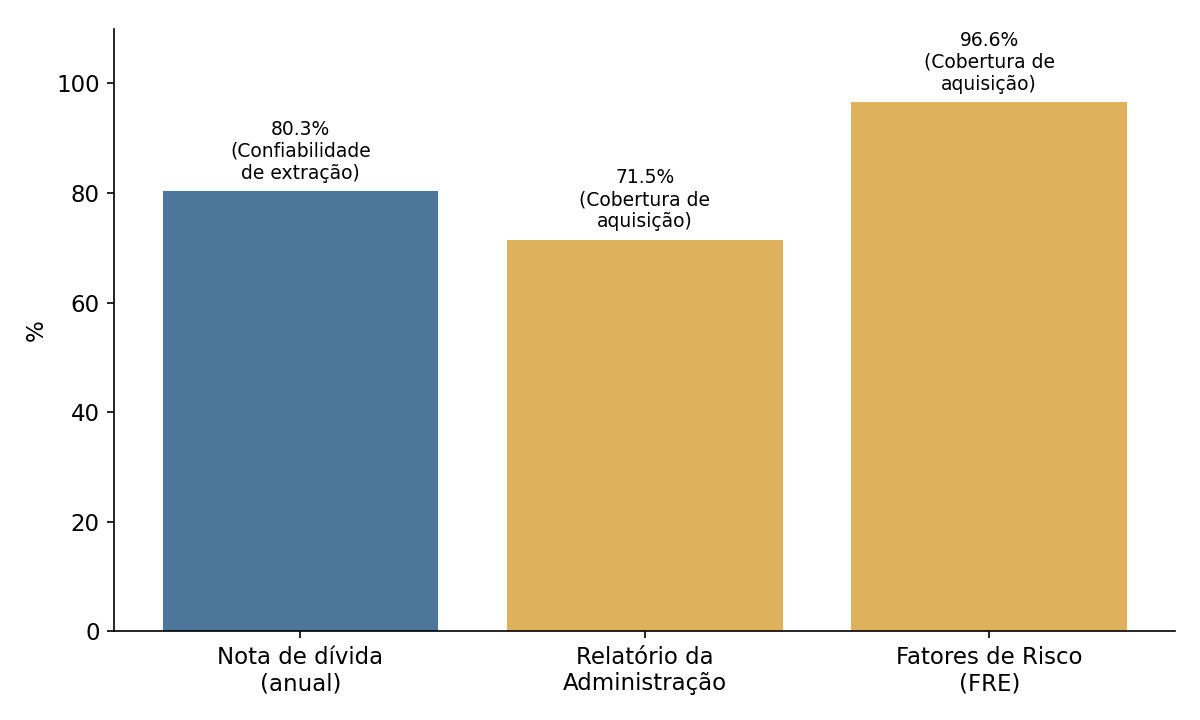
\includegraphics[width=0.8\textwidth]{figures/extraction_reliability.png}
    \caption{Confiabilidade de extração e cobertura de aquisição, por fonte de texto}
    \label{fig:confiabilidade}
    \vspace{0.2cm}

    {\footnotesize Fonte: elaborada pelo autor a partir dos logs de extração/aquisição do projeto.}
\end{figure}

A prática adotada ao longo de todo o projeto foi verificar cada padrão suspeito lendo diretamente uma amostra dos arquivos e casos concretos por trás dele, em vez de confiar apenas na estatística agregada. Essa prática, aplicada em rodadas de leitura e teste manual de exemplos, revelou problemas reais de qualidade de dados no cenário de conjunto completo de notas: alguns anexos capturados eram, na verdade, um documento diferente (por exemplo, um release de resultados em vez das demonstrações financeiras). Todos os resultados reportados no Capítulo~\ref{ch:resultados} usam apenas a versão já corrigida da aquisição.

\textbf{Regra metodológica: apenas extração confiável para a nota de dívida isolada.} A nota de dívida isolada é a única fonte de texto sujeita à heurística de localização de seção descrita acima, e portanto a única com uma classificação de confiabilidade (\textit{font\_heading} vs. \textit{regex\_only}) a considerar; as outras três fontes já chegam pré-isoladas, sem essa ambiguidade. A Seção~\ref{sec:poc_validacao} mostra que restringir a amostra a pares com \textit{font\_heading} nos dois anos desloca a distribuição de similaridade para um padrão mais bem comportado (Figura~\ref{fig:similaridade_bruta_confiavel}) sem alterar nenhuma conclusão de H1 ou H2. Diante disso, todos os resultados da nota de dívida isolada reportados a partir daqui -- Tabela~\ref{tab:sample} em diante, Capítulos~\ref{ch:resultados} -- usam exclusivamente essa amostra restrita, não mais o conjunto completo de pares computáveis.

\section{Estatísticas descritivas das variáveis}
\label{sec:estatisticas}

O número de pares ano a ano com similaridade textual calculável varia por fonte de texto, refletindo tanto as diferenças de cobertura da Seção~\ref{sec:confiabilidade} quanto o fato de as fontes mais recentes (conjunto completo de notas, Relatório da Administração, Fatores de Risco) terem sido incorporadas ao corpus em etapas posteriores do projeto (Tabela~\ref{tab:sample}).

\begin{table}[htbp]
    \centering
    \caption{Pares ano a ano por fonte de texto}
    \label{tab:sample}
    \begin{tabular}{@{}lrr@{}}
        \toprule
        \textbf{Fonte de texto} & \textbf{Pares} & \textbf{Empresas} \\
        \midrule
        Nota de dívida isolada (total)      & 1.858 & 177 \\
        \rowcolor{fontechave}
        \textbf{Nota de dívida isolada (confiável)}  & \textbf{1.426} & \textbf{166} \\
        Conjunto completo de notas explicativas & 1.933 & 178 \\
        Relatório da Administração & 1.340 & 160 \\
        Fatores de Risco (FRE) & 1.964 & 179 \\
        \bottomrule
    \end{tabular}
    \\[0.3cm]
    {\footnotesize Fonte: elaborada pelo autor a partir de dados da CVM, todos os pares em base anual. ``Total'' = todos os pares com similaridade computável; ``confiável'' = restrito a pares com extração confiável (\textit{font\_heading}) nos dois anos (Seção~\ref{sec:confiabilidade}), a amostra usada nos resultados a partir daqui. A linha em destaque (nota de dívida isolada, confiável) é a fonte de texto principal desta dissertação (Seção~\ref{sec:medida}); as demais são comparações de robustez e generalização (Seção~\ref{sec:identificacao}).}
\end{table}

Dados de mercado (preços diários da ação e do Ibovespa, 2010--2026, combinando a exportação original da Bloomberg com uma exportação mais recente e mais ampla que cobre o índice IBX inteiro) cobrem a totalidade das 185 empresas da amostra. Dados de consenso de EPS dos analistas (Bloomberg), usados na análise complementar de H2, cobrem 64 das 66 empresas atuais e 27 das 45 históricas; H2 permanece, por ora, restrita a esse universo de 111 empresas -- o consenso de EPS não foi reextraído para as 74 empresas IBX-extra nesta rodada de expansão.

A nota de dívida isolada em base anual é o objeto central desta dissertação (H1 e H2, Seção~\ref{sec:hipoteses}); as outras fontes de texto entram apenas como critério de comparação metodológica (Seção~\ref{sec:medida}), não como parte do teste das hipóteses. A Figura~\ref{fig:similaridade} compara a distribuição da similaridade de cosseno entre as quatro fontes, já sobre o universo expandido. Um padrão salta aos olhos e é relevante para a leitura dos resultados do Capítulo~\ref{ch:resultados}: o conjunto completo de notas e os Fatores de Risco concentram-se muito mais perto de 1 (mediana de 0,93 e 0,96, respectivamente) do que a nota de dívida isolada (mediana de 0,83, já sobre a amostra de extração confiável) e o Relatório da Administração (mediana de 0,84, o mais próximo da nota de dívida entre as quatro fontes). Ou seja, mesmo restrita à extração mais confiável, o recorte estreito da nota específica de dívida ainda captura mais mudança textual ano a ano do que o documento inteiro ou uma seção-padrão como Fatores de Risco, nos quais boilerplate estrutural dilui a mudança relativa; o Relatório da Administração, por ser também um texto mais narrativo e menos padronizado que uma nota contábil auditada, mostra um padrão de mudança textual mais parecido com o da nota de dívida do que com o dos outros dois.

\begin{figure}[htbp]
    \centering
    
\includegraphics[width=0.85\textwidth]{figures/similarity_by_source.png}
    \caption{Distribuição da similaridade textual ano a ano, por fonte}
    \label{fig:similaridade}
    \vspace{0.2cm}

    {\footnotesize Fonte: elaborada pelo autor. Caixas: 1º-3º quartil; linha central: mediana; pontos: valores atípicos.}
\end{figure}

A Figura~\ref{fig:retorno} mostra a distribuição do retorno anormal (variável dependente de H1, nota de dívida anual, $n=1.134$ pares, 142 empresas). É um subconjunto dos 1.426 pares com similaridade confiável da Tabela~\ref{tab:sample}: calcular o retorno anormal exige, adicionalmente, um ticker negociável e preço de mercado disponível no período, o que uma parte dos pares não tem (majoritariamente empresas históricas que saíram definitivamente do mercado, Seção~\ref{sec:amostra}). A mediana é de $-9{,}7\%$, sem assimetria extrema que por si só explicaria o resultado reportado no Capítulo~\ref{ch:resultados}. Um retorno anormal médio negativo é esperado em um mercado emergente com Ibovespa como referência em períodos de estresse macroeconômico (2015--2016, 2020) e, agora, também 2010--2013 e 2025 com a extensão do período, e não indica um problema de construção da variável.

\begin{figure}[htbp]
    \centering
    
\includegraphics[width=0.8\textwidth]{figures/abnormal_return_dist.png}
    \caption{Distribuição do retorno anormal (nota de dívida, base anual)}
    \label{fig:retorno}
    \vspace{0.2cm}

    {\footnotesize Fonte: elaborada pelo autor a partir de preços da Bloomberg. Percentis 1 e 99 truncados para legibilidade; estatísticas calculadas sobre a amostra de extração confiável.}
\end{figure}

As Figuras~\ref{fig:controles}, \ref{fig:controles_m2} e \ref{fig:controles_m3} mostram a distribuição das nove variáveis de controle da grade M0-M3 (Seção~\ref{sec:controles}), uma figura por bloco: a Figura~\ref{fig:controles} cobre os quatro fundamentos de nível que entram em M1 (tamanho, ROA, alavancagem, momento), sobre as 2.243 observações empresa-ano (179 empresas) com dados contábeis estruturados disponíveis -- um exercício fiscal individual por observação, e não um par ano a ano como nas contagens da Tabela~\ref{tab:sample}, o que explica o número maior; a Figura~\ref{fig:controles_m2} cobre as três mudanças contemporâneas de M2 ($\Delta$ROA, $\Delta$Alavancagem, $\Delta$Dívida); e a Figura~\ref{fig:controles_m3} cobre as duas variáveis de risco/retorno esperado de M3 (\textit{book-to-market} e volatilidade), ambas sobre a amostra da nota de dívida anual (extração confiável, $n=1.134$ pares). O logaritmo do ativo total tem distribuição aproximadamente normal, como esperado; alavancagem concentra-se abaixo de 1, com uma cauda de poucas empresas em dificuldade financeira severa (passivo superior ao ativo); ROA concentra-se perto de zero com cauda esquerda mais longa (empresas com prejuízo); e o retorno passado tem assimetria positiva característica de retornos de ações.

\begin{figure}[htbp]
    \centering
    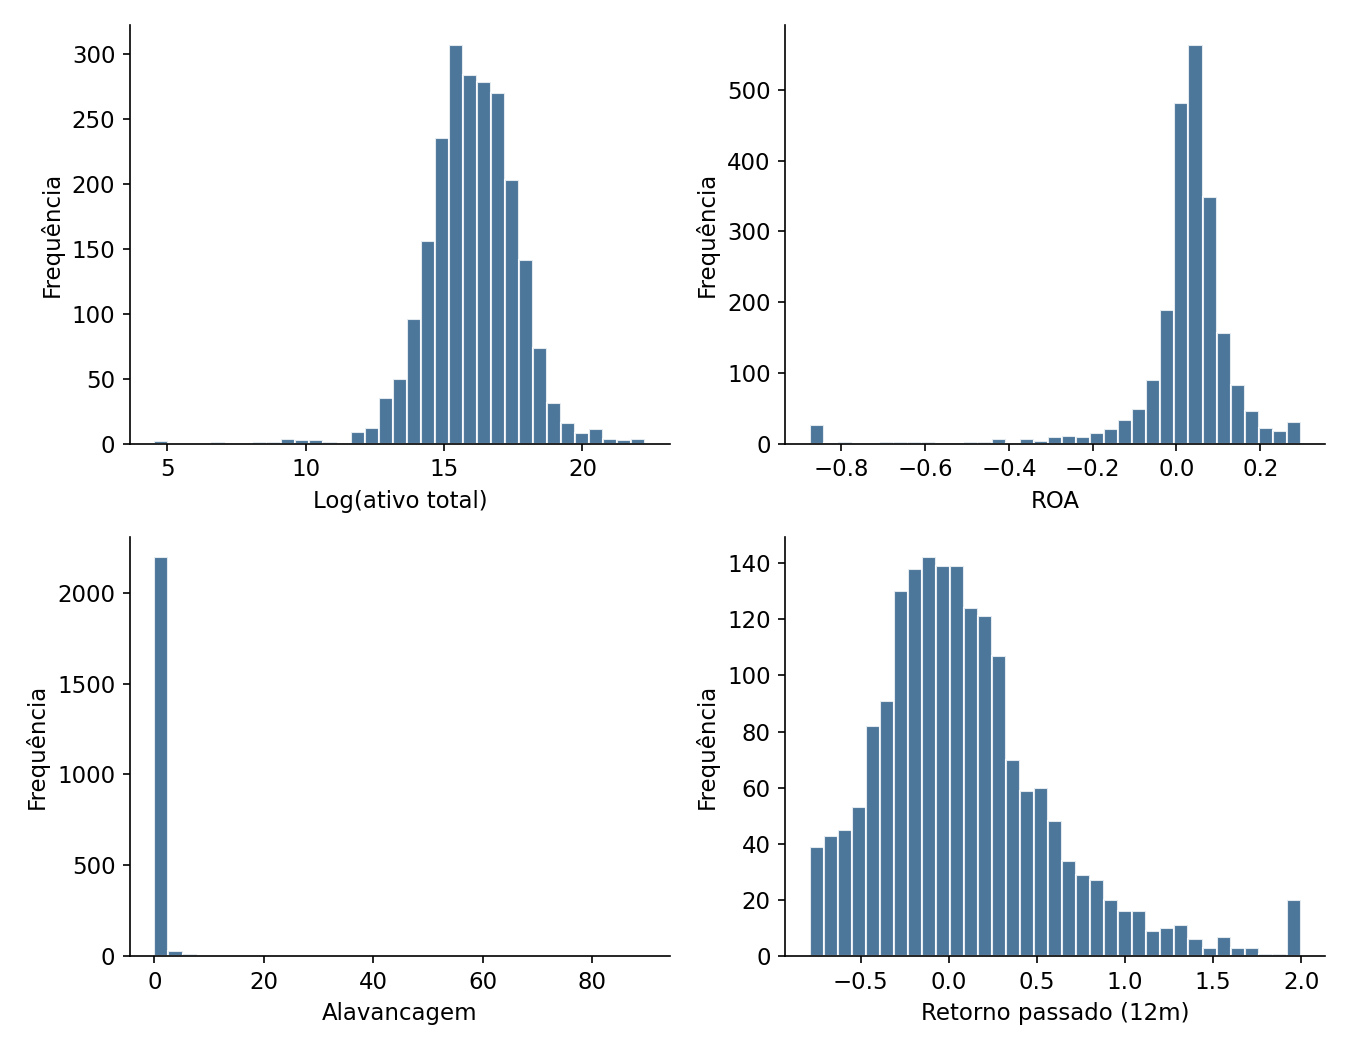
\includegraphics[width=0.62\textwidth]{figures/control_variables.png}
    \caption{Distribuição dos controles de nível (M1)}
    \label{fig:controles}
    \vspace{0.2cm}

    {\footnotesize Fonte: elaborada pelo autor a partir de dados contábeis estruturados da CVM. ROA e retorno passado truncados nos percentis 1/99 para legibilidade.}
\end{figure}

As três mudanças de M2 concentram-se perto de zero, como esperado para uma variação ano a ano em empresas maduras, com caudas moderadas nos dois sentidos (empresas em reestruturação financeira mais acentuada).

\begin{figure}[htbp]
    \centering
    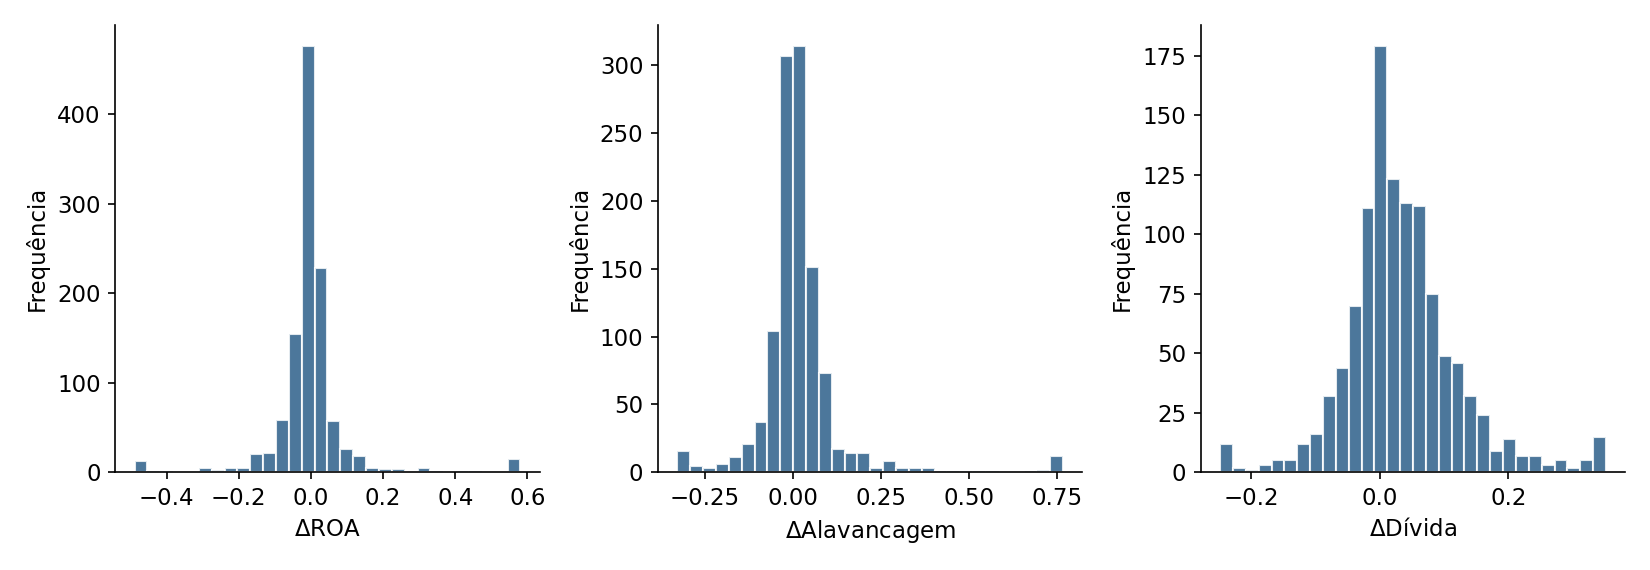
\includegraphics[width=0.95\textwidth]{figures/m2_controls.png}
    \caption{Distribuição dos controles de M2}
    \label{fig:controles_m2}
    \vspace{0.2cm}

    {\footnotesize Fonte: elaborada pelo autor a partir de dados contábeis estruturados da CVM. Percentis 1/99 truncados para legibilidade.}
\end{figure}

O \textit{book-to-market} de M3 tem a assimetria positiva característica dessa variável (poucas empresas negociando muito abaixo do valor patrimonial, a maioria acima), consistente com o que a literatura reporta para outros mercados \cite{famafrench1992}, e a volatilidade de M3 concentra-se entre 1,5\% e 3,5\% de desvio-padrão diário, com uma cauda de empresas mais voláteis -- tipicamente aquelas atravessando dificuldade financeira ou operando em setores mais cíclicos no período.

\begin{figure}[htbp]
    \centering
    
\includegraphics[width=0.75\textwidth]{figures/m3_controls.png}
    \caption{Distribuição dos controles de M3}
    \label{fig:controles_m3}
    \vspace{0.2cm}

    {\footnotesize Fonte: elaborada pelo autor a partir de preços/indicadores de mercado da Bloomberg. Percentis 1/99 truncados para legibilidade.}
\end{figure}

A cobertura é alta nas cinco variáveis de M2/M3: 1.133 ou 1.134 de 1.134 pares (99,9\%) para as três mudanças contemporâneas e para a volatilidade, e 1.091 de 1.134 (96,2\%) para \textit{book-to-market}, cuja lacuna reflete casos sem cotação de preço-sobre-valor-patrimonial disponível na data de referência.

\chapter{Resultados}
\label{ch:resultados}

\textit{[Os resultados deste capítulo ainda são preliminares e sujeitos a ajuste.]}

\section{Validação da medida de mudança textual}
\label{sec:poc_validacao}

Antes dos testes confirmatórios de H1 e H2 (Seções~\ref{sec:h1_resultados}--\ref{sec:h2_resultados}), uma fase exploratória iterativa verificou se a similaridade TF-IDF aplicada à nota de dívida captura de fato conteúdo textual real, e não apenas ruído de extração. Essa validação não é, em si, um teste de hipótese; é o alicerce que dá suporte à leitura dos resultados das seções seguintes.

\textbf{Confiabilidade de extração ao longo das rodadas.} A Figura~\ref{fig:trajetoria_extracao} mostra a evolução da taxa de extração confiável (\textit{font\_heading}), rodada a rodada, a partir da rodada 4 -- a primeira rodada sobre o universo completo então disponível (111 empresas, 997 arquivamentos), e não sobre as subamostras como as rodadas 1--3. A rodada 4 estabeleceu a linha de base em 43,8\%; quatro aprimoramentos cumulativos, cada um motivado pela inspeção direta de casos reais de falha e validado contra controles já funcionais para garantir ausência de regressão, elevaram essa taxa para 69,7\% na rodada 6, ainda sobre o corpus de 997 arquivamentos. O maior ganho isolado até então veio do reconhecimento de títulos em negrito do mesmo tamanho da fonte do corpo do texto (não apenas maiores), que resolveu sozinho 22 empresas que tinham taxa de extração confiável de 0\% em todos os anos verificados.

A rodada 7, motivada pela expansão do universo para 185 empresas (Seção~\ref{sec:amostra}, 2.129 arquivamentos), avaliou primeiro a heurística da rodada 6 -- sem qualquer mudança de código -- sobre esse corpus maior, obtendo 77,5\% (a mudança de universo, por si só, não piora a confiabilidade; a diferença em relação aos 69,7\% da rodada 6 reflete uma correção de aquisição feita durante a mesma expansão, descrita na Seção~\ref{sec:confiabilidade}, aplicada retroativamente também ao corpus original). Sobre essa base já corrigida, um último aprimoramento de heurística reconheceu títulos com prefixo numerado e fonte claramente maior que o corpo do texto, mesmo sem negrito -- um estilo de título real, encontrado por inspeção do corpus expandido, não previsto pelas seis rodadas anteriores --, elevando a taxa final para 80,3\%.

\begin{figure}[htbp]
    \centering
    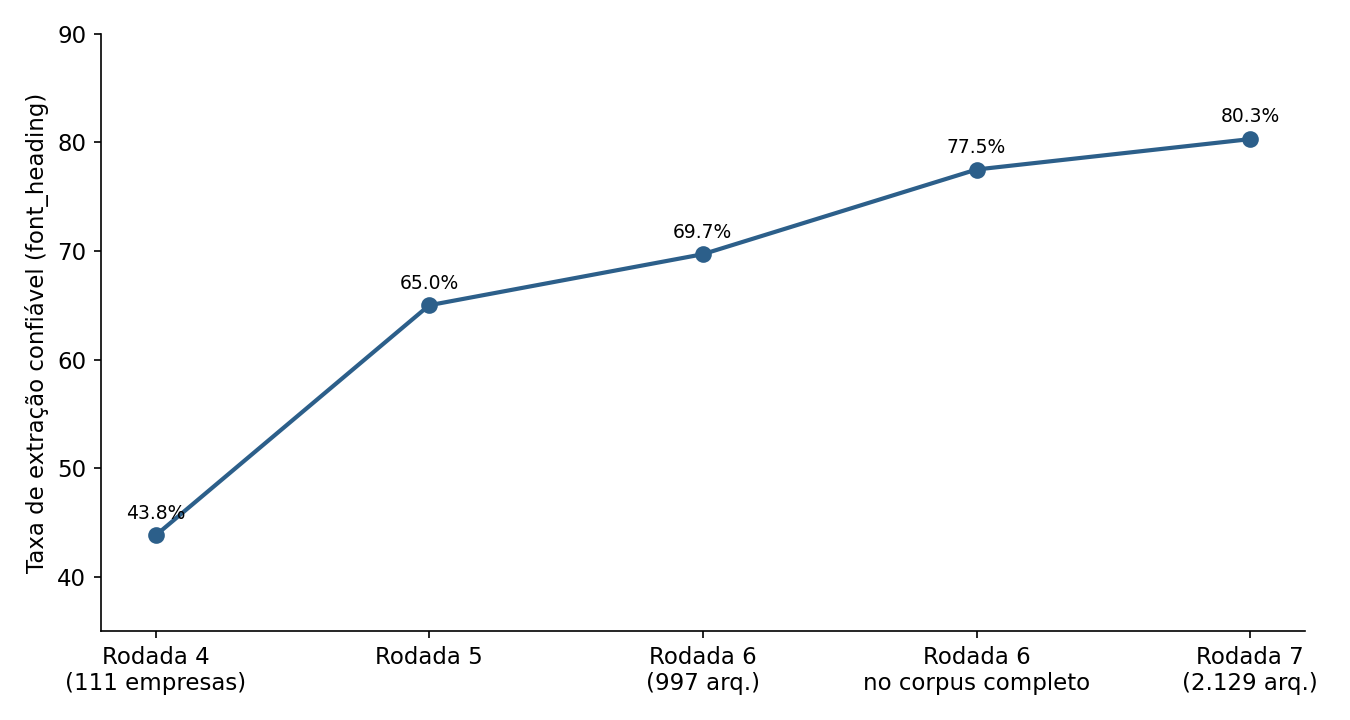
\includegraphics[width=0.85\textwidth]{figures/extraction_hardening_trajectory.png}
    \caption{Confiabilidade de extração ao longo das rodadas de aprimoramento}
    \label{fig:trajetoria_extracao}
    \vspace{0.2cm}

    {\footnotesize Fonte: elaborada pelo autor a partir dos logs de extração do projeto. Rodadas 4--6: corpus de 111 empresas (997 arquivamentos); rodada 7: corpus expandido de 185 empresas (2.129 arquivamentos).}
\end{figure}

\textbf{A similaridade se comporta melhor exatamente onde a extração é confiável.} A Figura~\ref{fig:similaridade_bruta_confiavel} compara a distribuição de similaridade sobre todos os pares extraídos com a distribuição restrita aos pares em que ambos os anos tiveram extração confiável, agora sobre o universo expandido. Restringir à extração confiável desloca a média de 0,62 para 0,72 e a mediana de 0,76 para 0,83, e reduz a concentração anômala de escores próximos de 0 e exatamente 1 que caracteriza os casos de falha de extração conhecidos (ver adiante). Esse é o padrão esperado se a medida estiver de fato lendo o texto da nota; não seria o padrão esperado se a variação observada fosse puramente ruído de extração. É essa evidência que motiva adotar a extração confiável como a amostra padrão da nota de dívida isolada em todo o restante do trabalho (Seção~\ref{sec:confiabilidade}), em vez de mantê-la apenas como um teste de robustez à parte.

\begin{figure}[htbp]
    \centering
    
\includegraphics[width=0.9\textwidth]{figures/similarity_raw_vs_reliable.png}
    \caption{Distribuição da similaridade textual: todos os pares vs. apenas extração confiável}
    \label{fig:similaridade_bruta_confiavel}
    \vspace{0.2cm}

    {\footnotesize Fonte: elaborada pelo autor a partir de \textit{similarity\_results\_full\_history.csv} (corpus anual completo, 185 empresas).}
\end{figure}

\textbf{Dois casos concretos.} WEG (2015$\to$2016, similaridade 0,9902) é um exemplo de similaridade genuinamente alta: a estrutura da nota é praticamente idêntica entre os dois anos, apenas valores e data mudam, o padrão de ``boilerplate atualizado com novos números''. Já a Yduqs (2017$\to$2018 e 2018$\to$2019, similaridade exatamente 1,0000 nos dois pares) é um exemplo de falha de extração: o localizador capturou por engano, nesses três exercícios, o mesmo parágrafo genérico de política contábil em vez da nota real. Todo escore degenerado (exatamente 0 ou 1) inspecionado neste projeto rastreou até uma falha de extração conhecida, não até uma falha da própria medida de similaridade.

\textbf{Checagem exploratória de plausibilidade econômica: saída do Ibovespa.} Como uma verificação adicional de que a medida capta algo economicamente sensato antes dos testes formais, comparou-se a similaridade textual de empresas que saíram do Ibovespa em algum momento do período (por delistagem, fusão ou reestruturação societária) com a das empresas que permaneceram, sobre pares com extração confiável em ambos os anos (Figura~\ref{fig:sobrevivencia}). Essa checagem, por depender de um desfecho (``saiu do Ibovespa'') que só é bem definido para empresas que em algum momento estiveram no índice, permanece restrita ao grupo original de 111 empresas (66 atuais + 45 históricas, Seção~\ref{sec:amostra}), não ao universo expandido de 185. A direção é a esperada pela lógica teórica do projeto (empresas em dificuldade tendem a mudar mais o texto da nota e também a sair do índice): mediana de 0,832 entre as que saíram contra 0,829 entre as que permaneceram. Sobre o universo completo e não enviesado desse grupo (192 pares de empresas que saíram, 335 de empresas que permaneceram), essa diferença não atinge significância convencional (Mann-Whitney unilateral, $p=0{,}359$), um resultado consistente com a checagem de deslistamento formal reportada na Seção~\ref{sec:robustez} para a nota de dívida isolada. O objetivo desta checagem exploratória era mostrar que a direção do efeito é a esperada teoricamente.

\begin{figure}[htbp]
    \centering
    
\includegraphics[width=0.7\textwidth]{figures/survivorship_boxplot.png}
    \caption{Similaridade textual: empresas que saíram do Ibovespa vs. que permaneceram}
    \label{fig:sobrevivencia}
    \vspace{0.2cm}

    {\footnotesize Fonte: elaborada pelo autor a partir de \textit{delisted\_similarity\_results.csv} (POC, pares com extração confiável em ambos os anos).}
\end{figure}

Em conjunto, essas três verificações (evolução da confiabilidade de extração, comportamento da distribuição de similaridade e plausibilidade econômica direcional) indicam que o pipeline de dados capta um sinal textual real. É sobre essa base que os testes formais de H1 e H2, a seguir, devem ser lidos: os resultados nulos das próximas seções indicam ausência de evidência de previsibilidade, não prova de sua inexistência.

\section{Resultados do modelo principal (H1)}
\label{sec:h1_resultados}

A Tabela~\ref{tab:h1} reporta o p-valor do coeficiente de TextChange sobre o BHAR ajustado (Seção~\ref{sec:var_dependente}), para cada fonte de texto, ao longo da grade M0-M3 (Seção~\ref{sec:controles}): M0 (TextChange isolado, com efeitos fixos de empresa e ano), M1 (mais tamanho, ROA, alavancagem e momento), M2 (mais as mudanças contemporâneas de ROA, alavancagem e dívida -- especificação principal) e M3 (mais \textit{book-to-market} e volatilidade).

\begin{table}[htbp]
    \centering
    \caption{Resultados do modelo principal (H1) por fonte de texto, grade M0-M3, universo expandido (185 empresas, 2010--2025)}
    \label{tab:h1}
    \small
    \begin{tabular}{@{}lrrrrr@{}}
        \toprule
        \textbf{Fonte de texto} & \textbf{n (M3)} & \textbf{M0} & \textbf{M1} & \cellcolor{m2principal}\textbf{M2*} & \textbf{M3} \\
        \midrule
        \rowcolor{fontechave}
        \textbf{Nota de dívida (anual)}       & \textbf{1.072} & \textbf{0,010} & \textbf{0,021} & \cellcolor{m2intersecao}\textbf{0,017} & \textbf{0,011} \\
        Conjunto completo de notas   & 1.445 & 0,737 & 0,638 & \cellcolor{m2principal}0,635 & 0,231 \\
        Relatório da Administração   & 1.013 & 0,510 & 0,685 & \cellcolor{m2principal}0,632 & 0,415 \\
        Fatores de Risco (FRE)       & 1.391 & 0,765 & 0,683 & \cellcolor{m2principal}0,781 & 0,751 \\
        \bottomrule
    \end{tabular}
    \\[0.3cm]
    {\footnotesize Fonte: elaborada pelo autor. Valores são p-valores de TextChange, erros-padrão agrupados por empresa. Destaques: M2, especificação principal; nota de dívida anual, fonte de texto principal. Detalhamento completo na Tabela~\ref{tab:h1_m2_detalhe}.}
\end{table}

Sobre o universo expandido, a nota de dívida anual -- a fonte de texto principal desta dissertação -- é a única a mostrar associação estatisticamente significativa entre TextChange e o retorno anormal, e o é em todo estágio da grade M0-M3, inclusive na especificação principal (M2: $\beta=0{,}156$, $p=0{,}017$) e na robustez econômica completa (M3: $p=0{,}011$). Nenhuma das outras três fontes mostra associação significativa em nenhum estágio, o mesmo padrão nulo já documentado na versão original da amostra (111 empresas, 2015--2024). Essa especificidade -- o efeito aparece exatamente na fonte teoricamente mais motivada (Seção~\ref{sec:medida}) e em nenhuma das três usadas como comparação metodológica -- é discutida com mais detalhe adiante nesta seção, depois do detalhamento de coeficientes a seguir, e é submetida à bateria de robustez completa na Seção~\ref{sec:robustez}. A Tabela~\ref{tab:h1_m2_detalhe} detalha o coeficiente, o erro-padrão e o intervalo de confiança de 95\% de cada modelo e cada fonte.

\begin{table}[htbp]
    \centering
    \caption{H1, grade M0-M3 completa: coeficiente, erro-padrão e IC 95\% por fonte de texto e modelo}
    \label{tab:h1_m2_detalhe}
    \small
    \begin{tabular}{@{}llrrrr@{}}
        \toprule
        \textbf{Fonte de texto} & \textbf{M} & \textbf{n} & \textbf{$\hat\beta$ (EP)} & \textbf{IC 95\%} & \textbf{p} \\
        \midrule
        Nota de dívida (anual)      & M0 & 1.134 & 0,165 (0,064) & [0,039; 0,291] & \textbf{0,010} \\
                                     & M1 & 1.115 & 0,151 (0,065) & [0,023; 0,279] & \textbf{0,021} \\
                                     & M2* & 1.115 & 0,156 (0,065) & [0,028; 0,284] & \textbf{0,017} \\
                                     & M3 & 1.072 & 0,170 (0,066) & [0,040; 0,300] & \textbf{0,011} \\
        Conjunto completo de notas  & M0 & 1.528 & $-$0,031 (0,091) & [$-$0,210; 0,148] & 0,737 \\
                                     & M1 & 1.505 & $-$0,042 (0,089) & [$-$0,217; 0,133] & 0,638 \\
                                     & M2* & 1.505 & $-$0,043 (0,089) & [$-$0,218; 0,133] & 0,635 \\
                                     & M3 & 1.445 & $-$0,108 (0,090) & [$-$0,284; 0,069] & 0,231 \\
        Relatório da Administração  & M0 & 1.081 & $-$0,086 (0,130) & [$-$0,342; 0,170] & 0,510 \\
                                     & M1 & 1.066 & $-$0,058 (0,142) & [$-$0,336; 0,221] & 0,685 \\
                                     & M2* & 1.066 & $-$0,068 (0,142) & [$-$0,346; 0,210] & 0,632 \\
                                     & M3 & 1.013 & $-$0,129 (0,158) & [$-$0,438; 0,181] & 0,415 \\
        Fatores de Risco (FRE)      & M0 & 1.456 & 0,044 (0,146) & [$-$0,244; 0,331] & 0,765 \\
                                     & M1 & 1.445 & 0,056 (0,137) & [$-$0,213; 0,325] & 0,683 \\
                                     & M2* & 1.445 & 0,039 (0,141) & [$-$0,237; 0,315] & 0,781 \\
                                     & M3 & 1.391 & 0,042 (0,134) & [$-$0,220; 0,305] & 0,751 \\
        \bottomrule
    \end{tabular}
    \\[0.3cm]
    {\footnotesize Fonte: elaborada pelo autor. EP = erro-padrão agrupado por empresa. *M2 é a especificação principal. Nota de dívida (anual): amostra restrita a pares com extração confiável (Seção~\ref{sec:confiabilidade}); é o único bloco de linhas cujo intervalo de confiança não contém zero em nenhum modelo da grade.}
\end{table}

Um padrão nos coeficientes (não apenas nos p-valores) vale registrar: o sinal de $\hat\beta$ é positivo -- mais mudança textual associada a mais retorno anormal futuro -- na nota de dívida anual e nos Fatores de Risco em todo M0-M3, e no conjunto completo de notas e no Relatório da Administração é negativo em todo M0-M3. Apenas o primeiro padrão é significativo; o sinal dos demais não é, por si, interpretado como achado (Seção~\ref{sec:leitura_beta}, ``Como ler $\beta$''). A inconsistência de sinal entre as fontes que não atingem significância é consistente com serem, nessas três, majoritariamente ruído amostral em torno de zero; já a nota de dívida anual mostra um coeficiente de sinal estável e significativo do diagnóstico (M0) até a robustez econômica completa (M3) -- a leitura mais favorável a H1 possível dentro da grade (Seção~\ref{sec:leitura_beta}).

O padrão de resultados por fonte de texto, incluindo essa especificidade, também não é aleatório em relação à teoria -- mas aponta em direções diferentes dependendo de qual dos dois estudos que motivam esta dissertação (Seção~\ref{sec:atencao}) serve de referência. \citeonline{amelzadeh2016} documentam, dentro do próprio 10-K americano, que a reação de preço é mais rápida ao texto mais lido e discricionário (MD\&A) do que às notas explicativas, e que é justamente nas notas -- o texto mais técnico e auditado -- que a mudança prevê retorno futuro: exatamente o padrão encontrado aqui, em que a nota de dívida (o texto mais formulaico e auditado entre os quatro testados) é a única fonte significativa, e o Relatório da Administração e os Fatores de Risco (as fontes de maior discricionariedade narrativa, adquiridas especificamente para testar essa previsão da literatura) permanecem nulos em todo M0-M3. \citeonline{cohen2020}, por outro lado, documentam dentro da própria amostra que o efeito se concentra em texto de alta discricionariedade gerencial (Risk Factors, MD\&A), o oposto do padrão encontrado aqui. Essa divergência entre \citeonline{cohen2020} e \citeonline{amelzadeh2016} -- e a convergência desta dissertação com o segundo, não o primeiro -- é retomada com mais profundidade no Capítulo~\ref{ch:conclusao}; ela não invalida o resultado -- a robustez do coeficiente na fonte principal é testada extensivamente na Seção~\ref{sec:robustez} --, e pesa a favor de uma leitura específica de mecanismo (atenção limitada operando sobre texto tecnicamente denso, não sobre texto de alta discricionariedade) em vez de uma leitura genérica de que "mudança textual prevê retorno".

O resultado da nota de dívida anual é o teste confirmatório pré-especificado desta dissertação para H1 (Seção~\ref{sec:hipoteses}); as outras três fontes servem como checagens de especificidade e generalização, não como testes independentes da mesma hipótese (Seção~\ref{sec:identificacao}). O resultado nulo dessas três fontes, por sua vez, admite mais de uma explicação, e esta dissertação não escolhe uma única entre elas sem evidência adicional: (i) o mercado brasileiro pode incorporar a informação dessas divulgações rapidamente, antes da janela medida em cada caso; (ii) a similaridade de cosseno sobre TF-IDF capta mudança lexical, não necessariamente novidade econômica; (iii) informação relevante já pode estar refletida em outras divulgações que chegam ao mercado antes (fatos relevantes, teleconferências, releases de resultado); e (iv) o efeito verdadeiro pode ser pequeno e o poder estatístico insuficiente para distingui-lo de zero nessas três fontes especificamente. Essas leituras são retomadas com mais profundidade no Capítulo~\ref{ch:conclusao}.

\section{Testes de robustez}
\label{sec:robustez}

\textbf{Bateria de robustez do resultado principal (nota de dívida anual, M2).} O único coeficiente significativo da Tabela~\ref{tab:h1} foi submetido à mesma bateria de robustez usada em todo achado deste projeto antes de ser aceito como candidato a resultado, não apenas reportado com seu p-valor de especificação única:
\begin{itemize}
    \item \textit{Excluindo similaridade degenerada.} Removendo os 32 pares com similaridade $\leq 0{,}001$ ou $\geq 0{,}999$ (Seção~\ref{sec:poc_validacao} -- escores que, historicamente neste projeto, rastreiam até falha de extração, não sinal real): $p=0{,}046$, $n=1{.}083$. Continua abaixo de 5\%.
    \item \textit{BHAR bruto, sem winsorização.} Usando o BHAR antes do ajuste de winsorização descrito na Seção~\ref{sec:var_dependente} (o mesmo BHAR cuja assimetria de $9{,}33$ motivou o ajuste): $p=0{,}031$. Também abaixo de 5\%, e na verdade mais forte, não mais fraco.
    \item \textit{Exclusão de uma empresa por vez (\textit{leave-one-company-out}).} Reestimando o modelo 141 vezes, removendo uma empresa por vez: o pior caso entre as 141 reestimativas é $p=0{,}047$ (ao remover a empresa de CD\_CVM 20168), ainda abaixo de 5\%. O resultado não depende de nenhuma empresa isolada.
\end{itemize}
Os três testes usam a mesma especificação M2 e o mesmo painel de efeitos fixos de empresa e ano com erros-padrão agrupados por empresa da Tabela~\ref{tab:h1}. O resultado sobrevive a todos, um padrão bem mais robusto do que os achados frágeis documentados nas subseções seguintes desta mesma seção (Relatório da Administração sob o desenho antigo; Fatores de Risco). Além dessa bateria, as duas próximas subseções -- portfólio calendário e o desenho de \citeonline{santoscoelho2018} -- aplicam métodos de identificação inteiramente diferentes ao mesmo universo expandido, e ambas corroboram o resultado, em vez de apenas repeti-lo sob a mesma especificação. Duas checagens permanecem no universo original de 111 empresas por razão estrutural, não por falta de tempo: a checagem de deslistamento (Tabelas~\ref{tab:delisting}--\ref{tab:riskfactors}), cujo desfecho (``saiu do Ibovespa'') só é definido para empresas que em algum momento pertenceram ao índice (Seção~\ref{sec:amostra}); e a análise complementar de H2 (Seção~\ref{sec:h2_resultados}), que depende de uma série de consenso de EPS ainda não reextraída para as 74 empresas IBX-extra.

Numa etapa exploratória anterior deste trabalho, com o retorno ajustado ao mercado sem beta (Seção~\ref{sec:var_dependente}) e um conjunto de controles aproximando controles já testados na literatura, o Relatório da Administração chegou a mostrar um coeficiente significativo numa única especificação ($p=0{,}031$). O indício não sobreviveu a efeitos fixos de empresa e ano ($p=0{,}478$) nem a um teste de portfólio calendário independente (melhor caso $p=0{,}276$), e não reaparece em nenhuma célula da grade M0-M3 sob a especificação definitiva de retorno anormal (Tabela~\ref{tab:h1}, $p \geq 0{,}78$ em todo M para o Relatório da Administração).

\textbf{Teste de portfólio calendário para a nota de dívida (universo expandido).} Como verificação independente da ameaça de observações repetidas (Seção~\ref{sec:identificacao}), aplicou-se à nota de dívida anual -- a fonte de texto principal -- o teste de portfólio calendário longo-curto: carteiras formadas mensalmente por similaridade (terços, mantidas por 12 meses, para casar com o horizonte do BHAR ajustado) têm seu retorno testado pelo alfa de um modelo de quatro fatores idêntico ao usado para construir a variável dependente (Seção~\ref{sec:var_dependente}). Sobre o universo expandido, o alfa anualizado é de $-11{,}4\%$ ($t=-3{,}27$, $p=0{,}0011$): abaixo do limiar de 1\%, mais forte ($p=0{,}0003$) ao excluir os 48 pares com similaridade degenerada (Seção~\ref{sec:poc_validacao}), e replicado com sinal e magnitude semelhantes na outra combinação de 12 meses testada (dois grupos em vez de três: $-10{,}8\%$, $p=0{,}0015$); as combinações de 3 e 6 meses de manutenção não mostram efeito ($p \geq 0{,}33$ em todas), o mesmo padrão específico ao horizonte de 12 meses já observado na versão original deste teste. O sinal do alfa (carteira comprada em alta similaridade, vendida em baixa similaridade) é negativo, ou seja, empresas com \emph{mais} mudança textual (baixa similaridade) têm retorno subsequente maior -- a mesma direção do coeficiente positivo de TextChange na Tabela~\ref{tab:h1_m2_detalhe}, obtida aqui por um método completamente diferente (portfólio calendário, teste de alfa de fatores, sem impor forma funcional linear à relação) sobre os mesmos dados. Esse resultado é uma corroboração independente do achado principal, não apenas uma repetição sob outra especificação: onde a versão original deste teste (111 empresas) só alcançava significância marginal ($p=0{,}058$) e não sobrevivia à exclusão de similaridade degenerada, a versão sobre o universo expandido é significativa a 1\% e se fortalece sob a mesma checagem.

\textbf{Checagem de associação com saída do índice (universo original, 111 empresas).} Testou-se, para cada fonte de texto, se TextChange está associado à saída subsequente da empresa do Ibovespa (Tabela~\ref{tab:delisting}). Como discutido na Seção~\ref{sec:amostra}, esse desfecho só é bem definido para empresas que em algum momento pertenceram ao índice, de modo que esta checagem permanece no grupo de 111 empresas e não se estende às 74 empresas IBX-extra.

\begin{table}[htbp]
    \centering
    \caption{Associação entre TextChange e saída do índice, por fonte de texto}
    \label{tab:delisting}
    \begin{tabular}{@{}lrr@{}}
        \toprule
        \textbf{Fonte de texto} & \textbf{Sem controles} & \textbf{Modelo principal (M2)} \\
        \midrule
        Nota de dívida (anual)      & 0,649 & 0,754 \\
        Conjunto completo de notas  & 0,086 & 0,370 \\
        Relatório da Administração  & \textbf{0,033} & 0,127 \\
        \bottomrule
    \end{tabular}
    \\[0.3cm]
    {\footnotesize Nota de dívida (anual): amostra restrita a pares com extração confiável (Seção~\ref{sec:confiabilidade}).}
\end{table}

O Relatório da Administração é, novamente, a única fonte com algum sinal sem controles, mas não sobrevive à adição dos controles de M2 (tamanho, ROA, alavancagem, momento e as três mudanças contemporâneas). Efeitos fixos não foram aplicados a essa checagem especificamente: a condição de deslistamento é constante dentro de cada empresa, e a transformação de efeitos fixos elimina exatamente a variação que se quer explicar -- estimar o modelo mesmo assim produz um coeficiente de ordem $10^{-17}$ (essencialmente zero de máquina) acompanhado de um p-valor de 0,0057, que pareceria altamente significativo se lido sem esse cuidado.

\textbf{Achado adicional: Fatores de Risco e saída do índice, com desenho corrigido (universo original, 111 empresas).} Também não reestimado sobre o universo expandido, pela mesma razão da Tabela~\ref{tab:delisting}. A checagem de deslistamento é, por natureza, uma pergunta no nível da empresa, não no nível do par ano a ano: o desenho tecnicamente correto é uma única observação por empresa. Construiu-se uma variável de TextChange média por empresa, com os controles de M2 também agregados por empresa (média entre pares), e estimou-se uma regressão puramente transversal (Tabela~\ref{tab:riskfactors}).

\begin{table}[htbp]
    \centering
    \caption{Fatores de Risco e saída do índice: desenho transversal}
    \label{tab:riskfactors}
    \begin{tabular}{@{}p{6.5cm}rrr@{}}
        \toprule
        \textbf{Especificação} & \textbf{n} & \textbf{Coef.} & \textbf{p-valor} \\
        \midrule
        Sem controles                              & 94 & $1{,}99$ & \textbf{0,011} \\
        Modelo principal (M2), MQO                  & 94 & $1{,}76$ & \textbf{0,026} \\
        Modelo principal (M2), logit                & 94 & $15{,}71$ & \textbf{0,015} \\
        \bottomrule
    \end{tabular}
    \\[0.3cm]
    {\footnotesize $n=94$, não 110: 16 empresas perdem cobertura ao exigir os sete controles de M2 (sobretudo $\Delta$Dívida, que depende de dois exercícios consecutivos de dados contábeis).}
\end{table}

O coeficiente é positivo e consistente com a direção esperada: maior TextChange médio (mais mudança textual) associa-se a maior probabilidade de saída do índice. Diferentemente do achado do Relatório da Administração, este desenho não sofre do problema de observações repetidas em primeiro lugar, de modo que não há um teste mais rigoroso disponível capaz de invalidá-lo pela mesma via. O resultado sobrevive à troca do conjunto de controles original pelos controles de M2, teoricamente justificados. Mas a robustez não é completa: sob os controles de M2, a exclusão de cada empresa individualmente produz um pior caso de $p=0{,}107$, e substituir a média por mediana na agregação por empresa dá $p=0{,}120$ -- ambos acima do limiar de 5\%, diferente do que se observava sob o conjunto de controles antigo (pior caso $p=0{,}078$; mediana $p=0{,}033$). O achado central permanece significativo na especificação principal, mas é mais sensível a essas perturbações do que parecia antes.

\textbf{Comparação direta com o desenho de \citeonline{santoscoelho2018} (universo expandido).} Como verificação adicional, motivada diretamente pela limitação que os próprios autores apontam (Seção~\ref{sec:identificacao}), o modelo de retorno anormal foi reestimado seguindo o desenho metodológico deles o mais de perto possível: efeito único de empresa (sem efeito de ano), escolhido por teste de Hausman a cada especificação (efeitos fixos quando o teste rejeita a hipótese nula de equivalência, efeitos aleatórios caso contrário), com erros-padrão robustos à heterocedasticidade em vez de agrupados por empresa, com TextChange e o BHAR ajustado (Seção~\ref{sec:var_dependente}) no lugar da similaridade e do retorno ajustado ao mercado. A diferença deliberada em relação ao desenho original dos autores é o painel: dezesseis exercícios (2010--2025) em vez de três, permitindo que o teste de Hausman discrimine com mais confiança entre as duas abordagens (Tabela~\ref{tab:santoscoelho}).

\begin{table}[htbp]
    \centering
    \caption{Retorno anormal sob o desenho metodológico de Santos e Coelho (2018), universo expandido}
    \label{tab:santoscoelho}
    \small
    \resizebox{\textwidth}{!}{%
    \begin{tabular}{@{}llrrrrl@{}}
        \toprule
        \textbf{Fonte de texto} & \textbf{Janela} & \textbf{Ef. fixos (2 vias)} & \textbf{FE (só empresa)} & \textbf{RE (só empresa)} & \textbf{Hausman} & \textbf{Escolhido} \\
        \midrule
        \rowcolor{fontechave}
        \textbf{Nota de dívida (anual)}      & \textbf{12m} & \textbf{0,016} & \textbf{0,024} & \textbf{0,080} & \textbf{0,109} & \textbf{RE: 0,080} \\
        \rowcolor{fontechave}
                                     & \textbf{18m} & \textbf{0,006} & \textbf{0,008} & \textbf{0,043} & \textbf{0,347} & \textbf{RE: 0,043} \\
        Conjunto completo de notas  & 12m & 0,629 & 0,639 & 0,657 & 0,164 & RE: 0,657 \\
                                     & 18m & 0,728 & 0,796 & 0,936 & 0,000 & FE: 0,796 \\
        Relatório da Administração  & 12m & 0,748 & 0,828 & 0,119 & 0,000 & FE: 0,828 \\
                                     & 18m & 0,379 & 0,146 & 0,867 & 0,021 & FE: 0,146 \\
        Fatores de Risco            & 12m & 0,700 & 0,739 & 0,743 & 0,033 & FE: 0,739 \\
                                     & 18m & 0,742 & 0,480 & 0,490 & 0,027 & FE: 0,480 \\
        \bottomrule
    \end{tabular}%
    }
    \\[0.3cm]
    {\footnotesize Fonte: elaborada pelo autor. Valores são p-valores do coeficiente de TextChange, exceto a coluna Hausman (p-valor do teste de especificação) e a última coluna, que reporta o estimador escolhido pela regra de \citeonline{santoscoelho2018} (Hausman rejeita a 5\% $\rightarrow$ efeitos fixos; caso contrário, efeitos aleatórios) e o p-valor correspondente. Nota de dívida (anual): amostra restrita a pares com extração confiável (Seção~\ref{sec:confiabilidade}).}
\end{table}

A nota de dívida anual é, de novo, a única fonte com significância a 5\% -- em ambas as janelas testadas e em três das quatro colunas de cada linha (a exceção sendo o teste de Hausman em si, que não rejeita a hipótese de equivalência entre FE e RE em nenhuma das duas janelas, de modo que o estimador escolhido pela regra dos autores é o de efeitos aleatórios, mais eficiente: $p=0{,}080$ aos 12 meses, $p=0{,}043$ aos 18 meses). Nenhuma das outras três fontes mostra significância em nenhuma janela ou coluna, o mesmo padrão de especificidade já visto na Tabela~\ref{tab:h1}.

Esse exercício responde diretamente à limitação que os autores apontam em seu próprio estudo: um painel mais longo, dizem eles, poderia revelar diferenças relevantes entre as abordagens de efeito fixo e aleatório que um painel curto não capta com confiança. Um painel mais de cinco vezes mais longo (dezesseis exercícios contra três) permite exatamente esse teste com mais poder estatístico -- e, diferentemente do que se observava sobre o universo original de 111 empresas (onde o resultado permanecia nulo sob este desenho), o resultado aqui confirma, por um terceiro método independente (após a regressão M2 e o portfólio calendário), que a associação entre mudança textual da nota de dívida e retorno anormal sobrevive a uma escolha de efeitos bem mais permissiva que a adotada como padrão nesta dissertação (Seção~\ref{sec:identificacao}). Isso não invalida a contribuição de \citeonline{santoscoelho2018}, que trata de uma pergunta diferente (valor de mercado corrente, não retorno futuro) com um recorte amostral diferente; mas sugere que a robustez do resultado principal não é um artefato da escolha específica de efeitos fixos de duas vias desta dissertação, nem da amostra de 111 empresas em que ele foi originalmente detectado.

\textbf{TF-IDF sem informação futura (universo expandido).} Como registrado na Seção~\ref{sec:medida}, ajustar o IDF sobre o corpus inteiro (2010--2025) levanta uma preocupação de \textit{look-ahead}: a representação de uma nota antiga é influenciada pela frequência de palavras observada em notas futuras. Para testar diretamente essa preocupação, a similaridade da nota de dívida anual foi recalculada usando IDF em janela expansiva -- um ajuste por exercício corrente, usando apenas documentos disponíveis até aquele exercício, refeito uma vez para cada ano de referência do período em vez de um único ajuste sobre todo o período -- a granularidade máxima possível, já que a coleta é anual e o conjunto de documentos disponíveis não muda dentro de um mesmo exercício. A correlação entre a similaridade original e a recalculada é de $0{,}9992$ (diferença absoluta média de $0{,}006$ em uma escala de 0 a 1, essencialmente idêntica ao $0{,}9993$ observado sobre o universo original), e reestimar H1 (grade M0-M3, BHAR ajustado) sobre a versão sem informação futura não altera nenhuma conclusão ($p=0{,}021$ em M2, contra $p=0{,}017$ na versão original -- ambos significativos a 5\%). A preocupação com \textit{look-ahead} é legítima em princípio, mas seu impacto prático nesta amostra, como na amostra original, é desprezível.

\section{Análise complementar (H2)}
\label{sec:h2_resultados}

Como análise complementar (Seção~\ref{sec:h2_metodologia}), testou-se se TextChange também se associa à revisão do consenso de EPS dos analistas em torno da data de divulgação, seguindo a mesma grade M0-M3 da Seção~\ref{sec:h1_resultados} para as três fontes de texto aplicáveis (nota de dívida anual já restrita à amostra de extração confiável, Seção~\ref{sec:confiabilidade}). Diferentemente de H1, esta análise permanece no universo original de 111 empresas/2015--2024 (Seção~\ref{sec:fontes}): o consenso de EPS da Bloomberg não foi reextraído para as 74 empresas IBX-extra nem para o período 2010--2014 nesta rodada de expansão. O resultado é um nulo limpo em toda a grade: nenhuma fonte atinge significância a 5\% em nenhum M (Tabela~\ref{tab:h2}); a Tabela~\ref{tab:h2_detalhe} traz o coeficiente, o erro-padrão e o intervalo de confiança de 95\% de cada célula.

\begin{table}[htbp]
    \centering
    \caption{Resultados da análise complementar (H2) por fonte de texto, grade M0-M3}
    \label{tab:h2}
    \small
    \begin{tabular}{@{}lrrrrr@{}}
        \toprule
        \textbf{Fonte de texto} & \textbf{n (M3)} & \textbf{M0} & \textbf{M1} & \textbf{M2*} & \textbf{M3} \\
        \midrule
        Nota de dívida (anual)       & 339 & 0,704 & 0,826 & 0,839 & 0,746 \\
        Conjunto completo de notas   & 316 & 0,913 & 0,897 & 0,932 & 0,780 \\
        Relatório da Administração   & 386 & 0,629 & 0,972 & 0,735 & 0,631 \\
        \bottomrule
    \end{tabular}
    \\[0.3cm]
    {\footnotesize Fonte: elaborada pelo autor. Valores são p-valores do coeficiente de TextChange, erros-padrão agrupados por empresa. *M2 é a especificação principal. Nota de dívida (anual): amostra restrita a pares com extração confiável (Seção~\ref{sec:confiabilidade}). Fatores de Risco não consta: a revisão de consenso não foi construída para essa fonte.}
\end{table}

\begin{table}[htbp]
    \centering
    \caption{H2, grade M0-M3 completa: coeficiente, erro-padrão e IC 95\% por fonte de texto e modelo}
    \label{tab:h2_detalhe}
    \small
    \begin{tabular}{@{}llrrrr@{}}
        \toprule
        \textbf{Fonte de texto} & \textbf{M} & \textbf{n} & \textbf{$\hat\beta$ (EP)} & \textbf{IC 95\%} & \textbf{p} \\
        \midrule
        Nota de dívida (anual)      & M0 & 344 & 0,206 (0,540) & [$-$0,858; 1,270] & 0,704 \\
                                     & M1 & 339 & 0,127 (0,576) & [$-$1,009; 1,262] & 0,826 \\
                                     & M2* & 339 & 0,118 (0,577) & [$-$1,018; 1,254] & 0,839 \\
                                     & M3 & 339 & 0,182 (0,562) & [$-$0,926; 1,290] & 0,746 \\
        Conjunto completo de notas  & M0 & 323 & 0,080 (0,731) & [$-$1,360; 1,520] & 0,913 \\
                                     & M1 & 316 & $-$0,093 (0,721) & [$-$1,514; 1,327] & 0,897 \\
                                     & M2* & 316 & 0,064 (0,745) & [$-$1,404; 1,532] & 0,932 \\
                                     & M3 & 316 & 0,221 (0,788) & [$-$1,331; 1,772] & 0,780 \\
        Relatório da Administração  & M0 & 391 & $-$0,388 (0,802) & [$-$1,965; 1,189] & 0,629 \\
                                     & M1 & 386 & 0,025 (0,717) & [$-$1,385; 1,435] & 0,972 \\
                                     & M2* & 386 & 0,236 (0,694) & [$-$1,130; 1,601] & 0,735 \\
                                     & M3 & 386 & 0,350 (0,729) & [$-$1,084; 1,784] & 0,631 \\
        \bottomrule
    \end{tabular}
    \\[0.3cm]
    {\footnotesize Fonte: elaborada pelo autor. EP = erro-padrão agrupado por empresa. *M2 é a especificação principal. Todos os intervalos de confiança contêm zero, em todo modelo e toda fonte.}
\end{table}

Uma bateria secundária de testes exploratórios (comparação de tercil de TextChange e uma checagem de deslistamento aplicada à revisão) produziu três células com $p<0{,}05$ em 56 testes -- um número próximo do esperado por acaso puro -- e nenhuma sobreviveu à inspeção (padrão de tercil não monotônico em duas, e a checagem de deslistamento perdendo significância sob agrupamento por empresa na terceira). Seu resultado qualitativo -- nulo, com achados isolados que não resistem a exame -- é o mesmo confirmado pelo teste central da Tabela~\ref{tab:h2}.

Vale lembrar que a limitação de mensuração da série de consenso, discutida na Seção~\ref{sec:h2_metodologia}, permanece em aberto: parte do nulo aqui reportado pode refletir essa limitação, não apenas ausência de relação real.

\chapter{Conclusão}
\label{ch:conclusao}

[PLACEHOLDER - Escrever após terminar a dissertação]

\bibliography{references}

% \appendix
% \chapter{Apêndice A}

\end{document}
